%This is a template for producing LIPIcs articles. 
%See lipics-manual.pdf for further information.
%for A4 paper format use option "a4paper", for US-letter use option "letterpaper"
%for british hyphenation rules use option "UKenglish", for american hyphenation rules use option "USenglish"
%for section-numbered lemmas etc., use "numberwithinsect"
%for enabling cleveref support, use "cleveref"
%for enabling cleveref support, use "autoref"

\documentclass[a4paper,UKenglish,cleveref,autoref]{lipics-v2019}

\graphicspath{{./img/}}%helpful if your graphic files are in another directory

\usepackage{amsmath,amssymb,amsthm}
\usepackage{stmaryrd}
\usepackage{listings,color}
\usepackage{alltt}
\usepackage{flushend}
\usepackage[utf8]{inputenc} % for proper diacritics: Universität, Hüttel, Luís
\usepackage[T1]{fontenc}
\usepackage{algorithm}
\usepackage[noend]{algpseudocode}
\usepackage{graphicx}
\usepackage{tikz-cd}
\usepackage{multicol, enumitem}

\usepackage[portuguese]{babel}
\usepackage[utf8]{inputenc}  % for proper diacritics
\usepackage[T1]{fontenc}
\usepackage {listings}
\usepackage{tikz}
% \usepackage{xcolor}
% Links
\usepackage{hyperref}

\usepackage{amsmath,amssymb}
%\usepackage{stmaryrd}
\usepackage{listings,color}
\usepackage{alltt}
\usepackage{flushend}



%\usepackage[T1]{fontenc}

% \lstdefinestyle{Go}{	
% 	keywordstyle=[1]\bfseries,
% 	basicstyle=\footnotesize\ttfamily,	
% 	numberstyle=\tiny,
% 	numbersep=5pt,
% 	breaklines=true,
% 	%prebreak=\raisebox{0ex}[0ex2][0ex]{\ensuremath{\hookleftarrow}},
% 	showstringspaces=false,
% 	upquote=true,
% 	tabsize=3,
% 	frame=tb,
% 	morekeywords={go,make,chan,int,import,main,func,for,select,case,string},
%       }

\lstdefinelanguage{Golang}%
  {morekeywords=[1]{package,import,func,type,struct,return,defer,panic,%
     recover,select,var,const,iota,},%
   morekeywords=[2]{string,uint,uint8,uint16,uint32,uint64,int,int8,int16,%
     int32,int64,bool,float32,float64,complex64,complex128,byte,rune,uintptr,%
     error,interface},%
   morekeywords=[3]{map,slice,make,new,nil,len,cap,copy,close,true,false,%
     delete,append,real,imag,complex,chan,},%
   morekeywords=[4]{for,break,continue,range,goto,switch,case,fallthrough,if,%
     else,default,},%
   morekeywords=[5]{Println,Printf,Error,Print,},%
   sensitive=true,%
   morecomment=[l]{//},%
   morecomment=[s]{/*}{*/},%
   morestring=[b]',%
   morestring=[b]",%
   morestring=[s]{`}{`},%
}

      
\lstdefinelanguage{SePi}%
  {morekeywords=[1]{type,integer,string,boolean,new, select, assume, assert},%
   sensitive=true,%
   morecomment=[l]{//},%
   morecomment=[s]{/*}{*/},%
   morestring=[b]',%
   morestring=[b]",%
   morestring=[s]{`}{`},%
 }

\lstdefinelanguage{CFST}%
{
  morekeywords=[1]{Int, Char, Bool, Skip, forall, rec, let, in, if, then, else, new, send, receive,
    select, fork, case, of, data, match, with},%  
  sensitive=true,%
  literate={->}{{$\rightarrow$}}1,%
   breaklines=true,
   morecomment=[l]{--},%
   morecomment=[s]{{-}{-}},%
   morestring=[b]',%
   morestring=[b]",%
   morestring=[s]{`}{`},%
 }

 

% notes
\newcommand{\todo}[1]{[{\color{blue}\textbf{#1}}]}

% Keywords
\newcommand{\keyword}[1]{\mathsf{#1}}

% Prekinds

\newcommand\prekind{\upsilon}

\newcommand{\stypes}{\mathcal S}
\newcommand\kinds{\stypes}

\newcommand{\types}{\mathcal T}
\newcommand\kindt{\types}

\newcommand\kindsch{\mathcal C}

% Multiplicity
\newcommand\Un{\ensuremath{\mathbf{u}}} % \infty
\newcommand\Lin{\ensuremath{\mathbf{l}}} % 1 

% Kinds
\newcommand\kind{\kappa}

% Grammars
\newcommand{\grmeq}{\; ::= \;}
\newcommand{\grmor}{\;\mid\;}

% type constructors
\newcommand\tcBase{B}
\newcommand\tcLolli\multimap
\newcommand\tcFun\to
\newcommand\tcBang{\mathop!}

% Keywords for types
\newcommand\kRec{\keyword{rec}}


% Types
\newcommand{\tskip}{\keyword{Skip}}
\newcommand\tSemi[2]{#1;#2}
\newcommand\tOut[1]{\tcBang#1}
\newcommand\tIn[1]{?#1}
\newcommand\tIChoice[1]{\oplus#1}
\newcommand\tEChoice[1]{\&#1}
\newcommand\tUnFun[2]{#1\tcFun#2}
\newcommand\tLinFun[2]{#1\tcLolli#2}
\newcommand\tPair[2]{#1\otimes#2}
\newcommand\tDatatype[1]{{[#1]}}
\newcommand\tRec[2]{\mu\,#1\,.\,#2}
\newcommand\tForall[2]{\forall\,#1\,.\,#2}

\newcommand\tRecK[2]{\kRec\,#1\,.\,#2}
% Environments
% \newcommand\emptyEnv{\cdot}
\newcommand\emptyEnv{\varepsilon}
\newcommand\kindEnv{\Delta}
\newcommand\varEnv{\Gamma}

% Language
% Expressions
% Language Types
\newcommand{\unite}{\keyword{Unit}}
\newcommand{\inte}{\keyword{Int}}
\newcommand{\chare}{\keyword{Char}}
\newcommand{\boole}{\keyword{Bool}}

% Variables
\newcommand\vare[1]{#1}
\newcommand\unlete[3]{\keyword{let} \; #1 = #2 \; \keyword{in} \; #3} 

% Applications
\newcommand\appe[2]{#1#2}
\newcommand\tappe[2]{#1[#2]}

% Conditional
\newcommand\conditionale[3]{\keyword{if}\;#1\;\keyword{then}\;#2\;\keyword{else} \; #3}

% Pairs
\newcommand\paire[2]{(#1,#2)}
\newcommand\binlete[4]{\keyword{let}\;#1, #2 = #3\;\keyword{in}\;#4}

% Session Types
\newcommand\newe[1]{\keyword{new}\;#1}
\newcommand\sende[2]{\keyword{send}\;#1\; #2}
\newcommand\recve[1]{\keyword{receive}\;#1}
\newcommand\selecte[1]{\keyword{select}\;#1}
\newcommand\matche[2]{\keyword{match}\;#1\;\keyword{with}\;#2}

% Fork
\newcommand\forke[1]{\keyword{fork}\;#1}

% Datatypes
\newcommand{\ctrcte}{C}
\newcommand\casee[2]{\keyword{case}\;#1\;\keyword{of}\;#2}

% Goal
\newcommand\Alg{\vdash_{a}}

% Equivalent
\newcommand\Equiv[2]{#1\,\thicksim\,#2}


%%% Local Variables:
%%% mode: latex
%%% TeX-master: "cfst-inforum18"
%%% End:
      

\title{Checking  the equivalence of context-free session types}

%optional, please use if title is longer than one line
\titlerunning{Checking  the equivalence of context-free session types}

\author{Bernardo Almeida}{LASIGE, Faculdade de Ciências, Universidade de Lisboa, Portugal}{balmeida@lasige.di.fc.ul.pt}{[funding]}{}

\author{Andreia Mordido}{LASIGE, Faculdade de Ciências, Universidade de Lisboa, Portugal}{afmordido@fc.ul.pt}{[funding]}{https://orcid.org/0000-0002-1547-0692}

\author{Vasco T. Vasconcelos}{LASIGE, Faculdade de Ciências, Universidade de Lisboa, Portugal}{vmvasconcelos@fc.ul.pt}{[funding]}{https://orcid.org/0000-0002-9539-8861}


%TODO mandatory, please use full name; only 1 author per \author macro; first two parameters are mandatory, other parameters can be empty. Please provide at least the name of the affiliation and the country. The full address is optional

\authorrunning{B. Almeida, A. Mordido and V.\,T. Vasconcelos}

\Copyright{Bernardo Almeida, Andreia Mordido, Vasco T.\ Vasconcelos}%TODO mandatory, please use full first names. LIPIcs license is "CC-BY";  http://creativecommons.org/licenses/by/3.0/

\funding{This work was supported by FCT through project Confident
  (PTDC/EEI-CTP/ 4503/2014) and the LASIGE Research Unit
  (UID/CEC/00408/2019).}%optional, to capture a funding statement, which applies to all authors. Please enter author specific funding statements as fifth argument of the \author macro.

\ccsdesc[100]{CCS →  Theory of computation →  Logic →  Type theory}
\ccsdesc[100]{CCS →  Theory of computation →  Formal languages and automata theory →  Grammars and context-free languages}%TODO mandatory: Please choose ACM 2012 classifications from https://dl.acm.org/ccs/ccs_flat.cfm 
%
\keywords{Types, Type equivalence, Bisimulation, Algorithm}%TODO mandatory; please add comma-separated list of keywords
%
%\category{}%optional, e.g. invited paper
%
%
%\supplement{}%optional, e.g. related research data, source code, ... 
%hosted on a repository like zenodo, figshare, GitHub, ...

%\acknowledgements{I want to thank \dots}%optional

\begin{document}

\maketitle

\begin{abstract}
  We present an algorithm to decide the equivalence of context-free
  session types, practical to the point of being incorporated in a
  compiler. We prove its soundness and completeness. We further study
  its behaviour in practice.

  % mandatory; please add comma-separated list of keywords
  \keywords{Types, Type equivalence, Bisimulation, Algorithm} 
\end{abstract}

  % Session types are paramount to describe the structured interaction
  % of processes via typed communication channels; however, they lack an
  % efficient description for serialization of tree-structured data in a
  % type-safe way.

  % Context-free session types were proposed as an extension of session
  % types able to capture the type-safe serialization of recursive
  % datatypes. For the sake of a practical usage, namely in the
  % definition of new programming languages, there is an urgent need for
  % an algorithm to decide type equivalence. In this work, we propose an
  % algorithm to decide type equivalence on context-free session
  % types. We prove its soundness and completeness, and validate the
  % algorithm on several examples.

%%% Local Variables:
%%% mode: latex
%%% TeX-master: "main"
%%% End:

\section{Motivation}
\label{sec:introduction}

Session types enhance the expressivity of traditional types for
programming languages by enabling describing structured communication
on heterogeneously typed
channels~\cite{DBLP:conf/concur/Honda93,DBLP:conf/esop/HondaVK98,DBLP:conf/parle/TakeuchiHK94}.
%
Traditional session types are \emph{regular}, in the sense that the
sequences of communication actions admitted by a type are in the union
of a regular language (for finite executions) and an $\omega$-regular
language (for infinite executions).
%
Introduced by Thiemann and Vasconcelos, context-free session types
liberate traditional session types from the shackles of tail
recursion, allowing for example, the safe serialization of arbitrary
recursive datatypes~\cite{thiemann2016context}.

If the algorithmic aspects of type equivalence for regular session
types are well known (Gay and Hole authored an algorithm to decide
subtyting~\cite{DBLP:journals/acta/GayH05}, from which type
equivalence can be derived), the same does not apply to context-free
session types.
%
In the aforementioned work, Thiemann and Vasconcelos showed that the
equivalence of context-free session types is decidable, by reducing
the problem to the verification of bisimulation for Basic Process
Algebra (BPA) which, in turn, was proved decidable by Christensen,
H{\"{u}}ttel, and Stirling~\cite{DBLP:journals/iandc/ChristensenHS95}.
%
Even if the equivalence problem for context-free session types is
known to be decidable, to date, no algorithm has been proposed for the
effect.

% Related work here

After the breakthrough by Christensen, H\"uttel, and Stirling--- a
result that provides no immediate practical algorithm---the problem of
deciding the equivalence of BPA terms has been addressed by several
researchers~\cite{DBLP:conf/mfcs/BurkartCS95,DBLP:journals/iandc/ChristensenHS95,janvcar1999techniques},
but again, no actual practical algorithm can be readily extracted from
these papers.
%
Furthermore, context-free session types are not necessarily normed,
which precludes using the original result by Baeten, Bergstra, and
Klop~\cite{baeten1993decidability}, as well as improvements by Janc\v
ar, Hirshfeld and
Moller~\cite{DBLP:journals/tcs/HirshfeldJM96,DBLP:conf/concur/HirshfeldM94}.

Our algorithm works along three stages.
%
The \emph{first stage} builds a context-free grammar in Greibach
Normal Formal (GNF)---in fact a simple grammar---from a context-free
session type in a way that bisimulation is preserved.  A basic result
from Baeten, Bergstra, and Klop states that any guarded BPA system can
be transformed in Greibach Normal Formal (GNF) while preserving
bisimulation equivalence, but unfortunately no procedure is
presented~\cite{baeten1993decidability}.
%
The \emph{second stage} prunes the grammar by removing unreachable
symbols in unnormed sequences of non-terminal symbols. This stage
builds on the result of Janc\v ar, Hirshfeld and Moller.
%
The \emph{third stage} constructs an expansion tree, by alternating
between expansion and simplification steps, using ideas from Janc\v
ar, Moller, and
Hirshfeld~\cite{hirshfeld1996bisimulation,janvcar1999techniques}.
%
\vv{mais trabalho relacionado aqui}

% Contributions
We present an algorithm to decide the equivalence of context-free
session types, practical to the point that it may be readily included
in any compiler, an exercise that we conducted in
parallel~\cite{freeST}.
%
The main contributions of this work are:
%
\begin{itemize}
\item The proposal and implementation of an algorithm to decide type
  equivalence of context-free session types (in 300 lines of Haskell
  code),
\item a proof of soundness and completeness of the algorithm against
  the declarative definition,
\item A study of the complexity of the algorithm,
\item The exploration of several optimizations that cut the running
  time in 12,000,000\%.
%\item validation of the algorithm on several meaningful examples.
\end{itemize}

% Outline

The rest of the paper is organized as follows: context-free session
types in Section~\ref{sec:contextfreesession}, the algorithm in
Section~\ref{sec:algorithm}, the main results in
Section~\ref{sec:soundness}, optimizations in
Section~\ref{sec:optimisations}, evaluation in
Section~\ref{sec:evaluation}, and conclusions in
Section~\ref{sec:conclusion}.

% Thiemann and
% Vasconcelos~\cite{thiemann2016context} proposed {\it context-free
%   session types} as an extension of session types by allowing nested
% protocols that are not restricted to tail recursion. Context-free
% session types capture the type-safe serialization of recursive
% datatypes and enable the type-safe implementation of remote operations
% on recursive datatypes.

% Inspired by the context-free session types' framework, Almeida and
% Vasconcelos~\cite{bernardo} proposed a functional programming language
% equipped with context-free session types.  Such a programming language
% is highly dependent on an algorithm to decide type equivalence. We
% have developed and implemented an algorithm to decide type
% equivalence. Our work capitalizes on the metatheory of context-free
% session types proposed by Thiemann and
% Vasconcelos~\cite{thiemann2016context}, where type equivalence was
% proved to be decidable. Although the decidability of equivalence on
% context-free session types has been addressed in the
% literature~\cite{DBLP:journals/iandc/ChristensenHS95,janvcar1999techniques,thiemann2016context},
% to the best of our knowledge, no algorithm was ever implemented.
% % and a possible implementation was not obvious.

%%% Local Variables:
%%% mode: latex
%%% TeX-master: "main"
%%% End:

\section{Context-free session types}
\label{sec:contextfreesession}

This section briefly introduces context-free session types, based on
the work of Thiemann and Vasconcelos~\cite{thiemann2016context}.
%
The types we consider build upon a denumerable set of \emph{variables}
and a set of \emph{choice labels}.  Metavariables $X,Y,Z$ range over
variables and $\ell$ over labels.
%
We assume given a set of base types denoted by~$B$.
% Further base types could include integer and boolean types, or any
% other type for which equality is decidable.
The syntax of types is given by the grammar below.
%
\begin{gather*}
  S,T \grmeq \skipk \grmor \sharp B \grmor 
  \star\{\ell_i\colon T_i\}_{i\in I} \grmor S;T \grmor \mu X.T \grmor X
  \\
  \sharp \grmeq {}! \grmor {}? 
  \qquad \qquad
  \star  \grmeq \oplus \grmor {}\&
  % \qquad \qquad
  % a \grmeq \sharp B \grmor \star l \grmor X
\end{gather*}

In type $\mu X.T$, variable $X$ is bound in the subterm~$T$. The sets
of bound and free variables in a given type are defined
accordingly. Notation $\subs{T}{X}S$ denotes the resulting of
substituting T for the (free) occurrences of $X$ in $S$.

Judgement $\DONE S$ characterizes \emph{terminated} types:
context-free session types that exhibit no further
action~\cite{DBLP:journals/jacm/AcetoH92}.

\noindent Terminated predicate:\hfill\fbox{$\DONE T$} 
%
\begin{gather*}
  \DONE{\skipk}
  \qquad 
  \DONE X
  \qquad
  \frac{\DONE{S} \quad \DONE{T}}{\DONE{S; T}}
  \qquad
  \frac{\DONE T}{\DONE{\mu X.T}}
\end{gather*}
%
Notice that all types of the form $\mu X. \mu X_1\dots\mu X_n.X$, for
$n\ge0$, are terminated.

We are not interested in all types generated by the above grammar.
%
If $\Delta$ is a list of pairwise distinct variables, then judgement
$\isType T$ characterises the types of interest: the
\emph{well-formed} types.

\noindent Type formation system: \hfill\fbox{$\isType T$}
%
\begin{gather*}
  \frac{} 
  {
    \isType \skipk
  }
  \enspace\;
  \frac{}
  {
    \isType {\sharp B}
  }
  \enspace\;
  \frac{
    X \in \Delta
  }{
    \isType{X}
  }
  \enspace\;
  \frac{
    \isType{S}
    \enspace
    \isType{T}
  }{
    \isType{S;T}
  }
  \enspace\;
  \frac{
    \isType{T_i}
    \enspace
    (\forall i\in I)
  }{
    \isType{\star 
      \{ \ell_i \colon T_i\}_{i\in I}}
  }
  \enspace\;
  \frac{
    % \isContr T
    \neg\DONE T
    \enspace 
    \isType [\Delta, X] T
  }{
    \isType {\mu X. T}
  }
\end{gather*}

Terminated processes have a simple characterisation---types comprising
$\skipk$, $\mu$ and semicolon---which justifies the inclusion of
$\neg\DONE T$ in the rules for type formation (Thiemann and
Vasconcelos~\cite{thiemann2016context} introduce a contractive judgement
for the effect).
%
Type formation serves two main purposes: ensuring that all variables
introduced by $\mu$-types are pairwise distinct and that types
underneath a~$\mu$ are not terminated. This can be clearly seen by
formation rule for $\mu$-types, where notation $\Delta,X$ is
understood as requiring $X\notin\Delta$.
%
In the sequel we assume that all types are such that $\isType[] T$ and
denote by $\mathcal{T}$ the set such types.

The set of \emph{actions} is generated by the following grammar.
\begin{equation*}
  a \grmeq \sharp B \grmor \star \ell
\end{equation*}

The \emph{labelled transition system} (LTS) for context-free session
types is given by $\mathcal{T}$ as the set of \emph{states}, the
set of \emph{actions}, and the \emph{transition relation}
$S\LTSderives T$ defined by the rules below.

\noindent Labelled transition system:\hfill\fbox{$S \LTSderives T$}
%
\begin{gather*}
  \sharp B \LTSderives[\sharp B] \skipk
  \qquad
  % X \LTSderives[X] \skipk
  % \qquad
  \star\{\ell_i\colon T_i\}_{i\in I} \LTSderives[\star \ell_j] T_j\quad
  (j\in I)
  \\
  \frac{S \LTSderives S'}{S; T \LTSderives S';T}
  \qquad
  \frac{\DONE{S} \quad T \LTSderives T'}{S; T \LTSderives T'}
  \qquad
  \frac{\subs{\mu X.S}{X}S \LTSderives T}{\mu X.S \LTSderives T}
\end{gather*}

\emph{Type bisimulation} is defined in the usual way from the labelled
transition system~\cite{sangiorgi2014introduction}.
%
We say that a type relation $\mathcal R$ is a \emph{bisimulation} if,
whenever $S\mathcal RT$, for all~$a$ we have:
%
\begin{itemize}
\item for each $S'$ with $S \LTSderives S'$, there is $T'$ such that $T
  \LTSderives T'$ and $S'\mathcal RT'$, and
\item for each $T'$ with $T \LTSderives T'$, there is $S'$ such that $S
  \LTSderives S'$ and $S'\mathcal RT'$.
\end{itemize}
%
We say that two types are bisimilar, written $S \bisim T$, if there
is a bisimulation~$\mathcal R$ with $S\mathcal RT$.

%%% Local Variables:
%%% mode: latex
%%% TeX-master: "main"
%%% End:

\section{An algorithm to decide type bisimilarity}
\label{sec:algorithm}

% Recall the type bisimulation problem for context-free session types.

% \begin{quote}
%   Given context-free session types $S$ and $T$, the type equivalence
%   problem consists in deciding if types $S$ and $T$ are equivalent,
%   i.e., $S \TypeEquiv T$.
% \end{quote}

This section presents an algorithm to decide whether two types are in
a type bisimulation. In the process we also provide an algorithm to
decide the bisimilarity of simple context-free languages.
%
The algorithm comprises three stages:
%
\begin{enumerate}
\item Translate the two types to a simple grammar,
\item Prune unreachable symbols, and
\item Explore an expansion tree, alternating between simplification
  and expansion operations, until either finding an empty node---case
  in which it decides positively---or failing to expand all nodes---case
  in which it decides negatively.
\end{enumerate}

\paragraph{Translating types to grammars}

% GREIBACH NORMAL FORMS

Type variables~$X$ are the \emph{non-terminal symbols} and LTS
labels~$a$ are the \emph{terminal symbols}. Sequences of type
variables~$\vec X$ are called \emph{words}; $\varepsilon$ denotes the
empty word.
%
A context-free grammar in Greibach Normal Form is a pair
$(\vec X,\mathcal P)$ where~$\vec X$ is the \emph{start word}
and~$\mathcal P$ a \emph{set of productions} of the form
$Y \rightarrow a\vec Z$ (context-free session types do not require
productions of the form $Y \rightarrow\varepsilon$).
%
Due to the deterministic nature of context-free session types, the
grammars we are interested in are \emph{simple}: for each
non-terminal symbol~$Y$ and each terminal symbol~$a$, there is at most
one production of the form $Y \rightarrow a\vec Z$.

% GRAMMAR LTS

Grammars in Greibach normal form naturally induce a labelled
transition system by taking words~$\vec X$ for states, terminal
symbols~$a$ for actions, and $\LTSderivesP$, defined as
$X\vec Y\LTSderivesP \vec Z\vec Y$ when
$X \rightarrow a\vec Z \in \mathcal P$, for the transition relation.
The associated bisimilarity is denoted by $\ProdEquiv$.

% UNRAVEL

The \emph{unravelling} function on well-formed context-free session
types, taken from Thiemann and Vasconcelos~\cite{thiemann2016context},
is defined as follows.
%
\begin{align*}
  \Unravel(\mu X.T) & = \Unravel(\subs{\mu X.T}XT)
  \\
  \Unravel (S;T) &= \left\{%
  \begin{array}{ll}
    \Unravel(T) & \Unravel(S) = \skipk
    \\
    (\Unravel(S); T) & \Unravel(S) \ne \skipk
  \end{array}
                        \right.
  \\
  \Unravel (T) &= T \qquad \text{in all other cases}
  % \Unravel(\mu X.T) & = \Unravel\subs{\mu X.T}XT])
  % &
  % \Unravel (S;T) &= \Unravel(T) \quad (\Unravel(S) = \skipk)
  % \\
  % \Unravel (T) &= T \quad (\text{all other cases})
  % &
  % \Unravel (S;T) &=  \Unravel(S); T \quad (\text{otherwise})
\end{align*}
%
The function terminates under the assumption that types are well
formed. 
%Thiemann and Vasconcelos~\cite{thiemann2016context} show that
%$\Unravel$ yields a guarded type of the form $\skipk$, $\sharp B$,
%$\star\{\ell_i\colon S_i\}$, or a $;$-type that starts with one the
%these.

% TO GRAMMAR

Another function $\word$ builds a word from a type. In the process it updates a
global set $\productions$ of grammar productions. Word concatenation is
denoted by $\vec X\cdot\vec Y$.
%
\begin{align*}
  \word(\skipk) &= \Empty
  \\
  \word(S;T) &= \word(S) \cdot \word(T)
  \\
  \word(\sharp B) &=
     Y,
     \text{ setting } \productions := \productions \cup (Y \rightarrow \sharp B)
    && (Y\text{ fresh})
  \\
  \word(\star\{\ell_i\colon T_i\}_{i\in I}) &=
     Y,
    \text{ setting } \productions := \productions \cup \{Y \rightarrow\star \ell_i\cdot \word(T_i) \mid i\in I\}
    && (Y\text{ fresh})
  \\
  \word(X) &= X
  \\
  \word(\mu X.T) &= X
\end{align*}


The following lemma relates terminated types~$T$ to the result 
of a call to $\word(T)$. 

\begin{lemma}
  \label{lemma:terminated-togrammar}
  Let $\isType[] T$. Then, $\DONE T$ if and only if
  $\word(T) = \varepsilon$.
\end{lemma}
%
\begin{proof}
  The direct implication follows by rule induction on
  predicate~$\DONE$:
  \begin{itemize}
  \item Case $\DONE{\skipk}$: $\word(\skipk) = \varepsilon$.
  \item Case $\DONE{X}$: if $T\triangleq X$, then $\isNotType[]T$.
  \item Case $\DONE{S;T}$: by induction hypothesis over the 
    rule premises 
    $\DONE{S}$ and $\DONE{T}$,
    $\word(S) = \varepsilon$ and $\word(T) = \varepsilon$. Hence,
    $\word(S;T) = \varepsilon$.
  \item Case $\mu X.S$: if $T\triangleq \mu X.S$, then the hypothesis 
    $\DONE T$ and the rule premises of 
    hypothesis $\isType[]T$ are contradictory.
  \end{itemize}
  %
  Conversely, if $\word(T) = \varepsilon$, using the rules of the definition of
  $\word$ that produce the empty word:
  \begin{itemize}
  \item if $T\triangleq \skipk$, then we have $\DONE T$.
  \item if $T\triangleq U;V$,
    $\word(U) = \varepsilon$, and $\word(V) = \varepsilon$, then, by
    induction, we have $\DONE U$ and $\DONE V$. Hence, $\DONE T$.
  \item No other case in function $\word$ produces an empty word. \qed
  \end{itemize}
\end{proof}


% COLLECT

To define the translation of context-free session types to simple
grammars, assume that $\{\mu X_1.T_1,\dots,\mu X_n.T_n\}$ is the set
of all $\mu$-subterms in a given type~$T$. Further assume that $i<j$
whenever $X_j \in \free(\mu X_i.T_i)$. That is, the $\mu$-subterms are
topologically sorted with respect to their lexical nesting, innermost
subterms first.
%
Now we identify unrolled versions of the $\mu$-subterms.
%
\begin{align*}
  T_1' &= \subs{\mu X_n.T_n}{X_n}{ \cdots \subs{\mu X_2.T_2}{X_2}\subs{\mu X_1.T_1}{X_1}{T_1} }\\
  T_2' &= \subs{\mu X_n.T_n}{X_n}{ \cdots \subs{\mu X_2.T_1}{X_2}{T_2} }\\
       &\;\;\vdots \\
  T_n' &= \subs{\mu X_n.T_n}{X_n}{T_n} 
\end{align*}
%
Clearly each type $T_i'$ is closed (has no free variables).
Notice that if $T$ is a $\mu$-type, then $\mu X_n. T_n$ is T itself.

% THE TRANSLATION

Finally, given an initial set of productions $\productions_0$, function
$\grm$ translates a type $T$ into a grammar composed of a start word
and set of productions:
%
\begin{equation*}
  \grm(T,\productions_0) = (\word(T), \productions_n)
\end{equation*}
%
where each $\productions_i$ is computed by the following recurrence,
\begin{equation*}
  % \left\{
  %   \begin{array}{lll}
  %     \productions_{0} &= \productions\\
  %     \productions_i &= 
                       \productions_i' \cup \{X_i \rightarrow a_j\vec
                       Y_j \vec Z \mid (Z \rightarrow a_j \vec Y_j)\in
                       \productions_i'\} \text{ where }(Z \vec Z, \productions_i')=\grm(\Unravel(T_i'), \productions_{i-1})
    % \end{array}\right.
\end{equation*}

Notice that $\word(\Unravel(T_i'))$ is a non-empty word because of
Lemma~\ref{lemma:terminated-togrammar} and the fact that each $T_i'$
is non-terminated by hypothesis.  The function $\grm$ terminates on
all inputs (because recursion is always on subterms) and adds a finite
number of productions to the original set. Furthermore, due to the
deterministic nature of session types, the function returns a simple
grammar.

To run $\grm$ on two well-formed types proceed as follows: rename the
second type so that bound variables do not overlap with those of the
first; start with an empty set of productions; run the algorithm
consecutively on the two types to obtain two initial words and a
single set of productions.

\begin{example}
  \label{ex:productions}
  Consider the following pair of context-free session types.
  % 
  \begin{align*}
    S & \triangleq (\mu X_1. \&\{n: X_1;X_1;?\intk, \ell: ?\intk\});(\mu X_2. !\intk ; X_2;X_2)\\
    T & \triangleq (\mu Y_1. \&\{n: Y_1;Y_1, \ell: \skipk\};?\intk);(\mu Y_2. !\intk ; Y_2)
  \end{align*}
  % 
  Starting from the empty set of productions, running $\grm$
  consecutively on~$S$ and on~$T$ produces the following set of
  productions
  %
  \begin{align*}
    X_1 &\rightarrow \& n\, X_1 X_1 X_3 & X_3 &\rightarrow \,? \intk &
    Y_1 &\rightarrow \& n\, Y_1 Y_1 Y_3 & Y_2 &\rightarrow \,!\intk\, Y_2 
    \\
    X_1 &\rightarrow \& \ell\, X_4           & X_4 &\rightarrow \,? \intk &
    Y_1 &\rightarrow \& \ell \,Y_3           & Y_3 &\rightarrow \,? \intk
    \\
    X_2 &\rightarrow \,!\intk\, X_2 X_2
  \end{align*}
  %
  and two start words $X_1X_2$ and $Y_1Y_2$.
\end{example}

\paragraph{Pruning unnormed productions}

For $\vec a$ a word $a_1,\dots, a_n$ ($n\ge1$), write
$\vec Y \LTSderivesP[\vec a] \vec Z$ when
$\vec Y \LTSderivesP[a_1] \cdots \LTSderivesP[a_n] \vec Z$.
%
We say that $\vec Y$ is \emph{normed} when
$\vec Y \LTSderivesP[\vec a] \varepsilon$ for some~$\vec a$, and that
$\vec Y$ is \emph{unnormed} otherwise.
%
When $\vec Y$ is normed, the \emph{minimal path} of $\vec Y$ is the
shortest~$\vec a$ such that $\vec Y \LTSderivesP[\vec a]
\varepsilon$.
%
In this case, the \emph{norm} of $\vec Y$, denoted by $|\vec Y|$, is
the length of~$\vec a$.
%
% Using the same approach as~\cite{DBLP:journals/iandc/ChristensenHS95} on
% the definition of (un)normed processes, we say that a sequence of symbols
% $\vec Y$ is \emph{normed} if there are labels $a_1,\ldots, a_n$
% such that:
% \begin{equation}
% \label{eq:path}
% 	\vec Y \rightarrow a_1\enspace Y_1 \rightarrow \cdots \rightarrow a_n
% 	\rightarrow \varepsilon.
% \end{equation}
% $\vec Y$ is said to be \emph{unnormed} when it is not normed. If $\vec Y$
% is normed, we define its \emph{norm} as:
% \[ | \vec Y | = \underset{n}{\mathsf{min}} \{\vec Y \rightarrow a_1\enspace Y_1
% \rightarrow \cdots \rightarrow a_n \rightarrow \varepsilon \}.\]
% A \emph{minimal path} for a normed sequence of symbols $\vec Y$ is a sequence of
% labels $\vec a = a_1,\ldots,a_n$ as in~\eqref{eq:path} such that
% $n = | \vec Y |$. To ease notation, we will also represent~\eqref{eq:path} as
% $\vec Y \xrightarrow{\vec a} \varepsilon$.
%
As observed by Christensen, H\"uttel, and
Stirling~\cite{DBLP:journals/iandc/ChristensenHS95}, any unnormed word
$\vec Y$ is bisimilar to its concatenation with any other word, that
is, if $\vec Y$ is unnormed, then $\vec Y \ProdEquiv \vec Y \vec X$.
We use this fact to prune unreachable symbols in unnormed words. And
we do this in all productions.

%The code is in Listing~\ref{lst:prune}.

% \begin{lstlisting}[
%   caption={Haskell code for stage 2: pruning unnormed productions},
%   label={lst:prune},
%   captionpos=b
%   ]
% type Visited = Set.Set [TypeVar]

% prune :: Productions -> Productions
% prune p = Map.map (Map.map (pruneWord p)) p

% pruneWord :: Productions -> Word -> Word
% pruneWord p = foldr (\x ys -> if normed p x then x:ys else [x]) []

% normed :: Productions -> TypeVar -> Bool
% normed p x = isJust $ maybeNorm p [x]

% maybeNorm :: Productions -> [TypeVar] -> Maybe Int
% maybeNorm p = norm Set.empty
%   where
%   norm :: Visited -> [TypeVar] -> Maybe Int
%   norm _ [] = Just 0
%   norm v xs
%    | any (flip isSubsequenceOf xs) v = Nothing
%    | otherwise = fmap (+1) (Map.foldr (compose min) Nothing (norms v xs))
%   norms :: Visited -> [TypeVar] -> Map.Map Label (Maybe Int)
%   norms v xs = Map.map (norm (Set.insert xs v)) (transitions xs p)
% \end{lstlisting}

\begin{example}
  \label{ex:prune}
  Recall Example~\ref{ex:productions} and notice that $X_2$ and $Y_2$
  are both unnormed. Then, the last occurrence of $X_2$ in production
  $X_2 \rightarrow \,!\intk\, X_2 X_2$ is unreachable, hence we
  simplify the production to obtain $X_2 \rightarrow \,!\intk\, X_2$.
  % \begin{center}
  %   \begin{tabular}{l l l}
  %     \multicolumn{3}{c}{Pruned productions for type $S$}\\ \hline
  %     \multicolumn{3}{c}{Start word: $X_1X_4$}\\
  %     $X_1 \rightarrow \& \ell\, X_3$  &
  %     $X_1 \rightarrow \& n\, X_1 X_1 X_2$ &
  %     $X_2 \rightarrow \,? \intk$ 
  %     \\
  %     $X_3 \rightarrow \,? \intk$ &
  %     $X_4 \rightarrow \,!\intk\, X_4$
  %   \end{tabular}
  % \end{center}
\end{example}

\paragraph{Building an expansion tree}

% We recall that, given two context-free session types $S$ and $T$, our main goal
% is to decide whether these types are equivalent or not. For this purpose,
% the algorithm we propose starts by applying algorithm presented in
% Listing~\ref{lst:toGrammar} to convert $S$ and $T$ into a grammar containing
% the productions derived from them. Afterwards, the algorithm in
% Listing~\ref{lst:prune} is used to streamline the grammars, by pruning
% unnormed sequences of symbols. Throughout this section we focus on the
% third and last step of the algorithm.

We base the third stage of the algorithm on the notion of
\emph{expansion tree} as proposed by Jan{\v{c}}ar and
Moller~\cite{janvcar1999techniques}, adapting an idea by
Hirshfeld~\cite{hirshfeld1996bisimulation}. The \emph{nodes} in trees
are labelled by sets of pairs of words.
%
We say that a node $N'$ is an \emph{expansion} of $N$ if $N'$ is a
minimal set such that: for every pair $(\vec X, \vec Y) \in N$,
\begin{itemize}
\item if $\vec X \rightarrow a\vec X'$ then
  $\vec Y \rightarrow a\vec Y'$ with $(\vec X',\vec Y')\in N'$, and
\item if $\vec Y \rightarrow a\vec Y'$ then
  $\vec X \rightarrow a \vec X'$ with $(\vec X',\vec Y')\in N'$.
\end{itemize}

An \emph{expansion tree} is built from a root node: the singleton set
containing the pair of start words obtained by translating the two
types into a grammar. A children node is obtained from its parent
node by expansion. However, as Jan{\v{c}}ar and Moller observed, expansions
alone often lead to infinite trees. We then alternate between
expansion and simplification operations, until either finding an empty
node---case in which we decide equivalence positively---or failing to
expand all nodes---case in which we decide equivalence negatively.
%
% The na\"ive proposal for an expansion tree considers that any
% children node is obtained by expansion from its parent
% node. Nevertheless, as Jan{\v{c}}ar and Moller observed, this would
% often lead to infinite expansion trees. Hence, we follow the
% proposal in~\cite{janvcar1999techniques} and let the expansion tree
% alternate between simplification and expansion operations until
% either finding an empty node---case in which we decide equivalence
% positively---or failing to expand a node---case in which we decide
% equivalence negatively.
%
We say that a branch is \emph{successful} if it is infinite or
finishes in an empty node, otherwise it is said to be
\emph{unsuccessful}.

%\paragraph*{Expansion step}
In the \emph{expansion step}, each node $N$ derives a single child
node, obtained as an expansion of $N$. As we are dealing with simple
grammars, no branching is expected in the expansion tree at this
step.
%

% \paragraph*{Simplification step}
The \emph{simplification step} consists on the application of the
following rules:
%
\begin{description}
\item[Reflexive rule:] Omit from a node any pair of the form
  $(\vec X,\vec X)$;
\item[Congruence rule:] Omit from a node $N$ any pair that belongs to
  the least congruence containing the ancestors of $N$;
  % \item {\bf Basic Process Algebra rules:} create sibling nodes for $N$
  % according to the following rules:
  % \begin{description}
\item[BPA1 rule:] If $(X_0 \vec X, Y_0 \vec Y)$ is in
  $N$ and $(X_0 \vec {X'}, Y_0 \vec {Y'})$ belongs to the ancestors of
  $N$, then create a sibling node for $N$ replacing
  $(X_0 \vec X, Y_0 \vec Y)$ by $(\vec X, \vec {X'})$ and
  $(\vec Y, \vec {Y'})$;
\item[BPA2 rule:] If $(X_0 \vec X, Y_0 \vec Y)$ is in $N$
  and $X_0$ and $Y_0$ are normed, then:
  \begin{description}
  \item[Case $|X_0| \leq |Y_0|$:] Let $\vec a$ be a minimal path
    for $X_0$ and $\vec Z$ the word such that
    $ Y_0 \LTSderivesP[\vec a] \vec Z$. Add a sibling node for
    $N$ including the pairs $(X_0 \vec Z, Y_0)$ and
    $(\vec X, \vec Z \vec Y)$ in place of $(X_0 \vec X, Y_0 \vec Y)$;
%  \item[Case] $|X_0| > |Y_0|$: Let $\vec a$ be a minimal path for 
  \item[Otherwise:] Let $\vec a$ be a minimal path for 
    $Y_0$ and $\vec Z$ the word such that
    $ X_0 \LTSderivesP[\vec a] \vec Z$. Add a sibling node for $N$
    including the pairs $(X_0 , Y_0 \vec Z )$ and
    $(\vec Z\vec X, \vec Y)$ in place of $(X_0 \vec X, Y_0 \vec Y)$.
  \end{description}
%		  \end{description}
%	\item {\bf Filtering rule:} remove any node containing a pair
%	       $(\vec X, \vec Y)$ such that $|\vec X|\neq |\vec Y|$.
\end{description}

Contrarily to expansion and to the reflexive and congruence
simplifications, \BPA\ rules promote branching in the expansion
tree. 
The application of these simplification rules is done iteratively,
to ensure the algorithm computes 
the simplest possible children nodes
derived from $N$. We showed that the simplification function that
results from applying the reflexive, congruence, and \BPA\ 
rules, has a fixed point in the complete partial ordered set of
pairs node-ancestors, where the set of ancestors is fixed.
The number of children nodes generated by the application 
of these rules was already proved to be
finite~\cite{DBLP:journals/iandc/ChristensenHS95,janvcar1999techniques}.
%
Notice that the sibling nodes do not exclude the
preservation of the (often) infinite
branch resulting from successive expansions.

\paragraph{Checking the bisimilarity of simple grammars}

Given a set of productions and two start words $\vec X$ and $\vec Y$
(all pruned), function $\Bisim$ alternates between simplification and
expansion stages, starting with expansion.
%
To avoid getting stuck in an infinite branch of the expansion tree, we
use a breadth-first search on the expansion tree: node-ancestor pairs
to be processed are stored in a queue. The initial pair inserted in the queue
contains the
initial node $\{(\vec X,\vec Y)\}$ and an empty set of ancestors.
%
\begin{equation*}
  \Bisim(\vec X, \vec Y, \productions) = \expand(
  \mathsf{singletonQueue}((\{(\vec X,\vec Y)\},\emptyset)),  
  \productions)
\end{equation*}

Predicate $\expand$ terminates as soon as all nodes fail to expand
(signaled by an empty queue), 
case in which the algorithm returns
$\False$, or an empty node is reached, case in which the algorithm
returns $\True$.
In the other cases, it identifies the front node in the queue, $n$,
and makes a recursive call after computing the nodes obtained by 
simplification from the child of $n$.
%
\begin{align*}
  &\expand(q, \productions) =\\
  &\quad \If\ \mathsf{empty}(q)\ \Then\ \False\\
  &\quad \Else\ (n,a) = \mathsf{front}(q)\\
  & \qquad\quad\; \If\ \mathsf{empty}(n)\ \Then\ \True\\
  & \qquad\quad\; \Else\ \If\ \mathsf{hasChild}(n, \productions)\\\
  & \qquad\qquad\quad\; \: \Then\
    \expand(\simplify(\mathsf{dequeue}(q), 
    \{(\mathsf{child}(n, \productions), a \cup n)\},\productions))\\
  & \qquad\qquad\quad\;\: \Else\ \expand(\mathsf{dequeue}(q), \productions)
\end{align*}

The simplification stage distinguishes the case where all type
variables are normed, in which case \BPA1 is not required to decide
equivalence~\cite{caucal1986decidabilite,DBLP:journals/iandc/ChristensenHS95},
from the case where some type variables might be unnormed.
%
\begin{align*}
  \mathsf{rules} =\;& \If\ \mathsf{allProductionsNormed(\productions)}\ \Then\
  [\mathsf{reflex} ,\mathsf{congruence}, \mathsf{bpa2}]\\
  &\Else\ [\mathsf{reflex} ,\mathsf{congruence}, \mathsf{bpa1} , \mathsf{bpa2}]
\end{align*}

Predicate $\simplify$ applies the various $\mathsf{rules}$ 
iteratively, until reaching a fixed point.
%
The application of the rules (via function
$\mathsf{apply}$) produces a set of nodes that
are then enqueued.
%
The simplification stage does not introduce new levels in the tree,
hence the set of ancestors $\mathit{na}$ is passed to function
$\mathsf{apply}$ as is.
%
\begin{align*}
  &\simplify(q, \mathit{na}, \productions) = \Fold(\mathsf{enqueue}, q,
    \mathsf{apply} (\mathit{na},
    \mathsf{rules}, \productions))
\end{align*}

% Given two context-free session types, function \lstinline|bisimilar|
% (in Listing~\ref{lst:algorithm}) starts by converting the two session
% types into a grammar, which is then pruned. Function
% \lstinline|convertToGrammar| (in Appendix) builds the initial monadic
% state, and runs the algorithm in Listing~\ref{lst:toGrammar} to
% convert the session types given as parameters.
% %
% An expansion tree is computed afterwards, through an alternation of
% expansion of children nodes and their simplification, using the
% reflexive, congruence, and \BPA\ rules.
% %
% \begin{lstlisting}[
%   caption={Haskell code for checking the bisimilarity of context-free
%     session types},
%   label={lst:algorithm},
%   captionpos=b
%   ]
% type Node = Set.Set (Word, Word)
% type Ancestors = Node
% type NodeQueue = Queue.Seq (Node, Ancestors)

% bisimilar :: TypeEnv -> Type -> Type -> Bool
% bisimilar tEnv t u = expand (xs, ys) (prune p)
%   where Grammar [xs, ys] p = trace (show t ++ "\nbisim\n" ++ show u) $ convertToGrammar tEnv [t, u]
        
% expand :: (Word, Word) -> Productions -> Bool
% expand p = expand' 1 (Queue.singleton (Set.singleton p, Set.empty))
%   where
%   expand' :: Int -> NodeQueue -> Productions -> Bool
%   expand' i ((n, a) Queue.:<| q) ps
%     | Set.null n      = True
%     | otherwise       = case expandNode ps n of
%         Nothing -> expand' (i+1) q ps
%         Just n' -> expand' (i+1) (simplify i ps n' (Set.union a n) q) ps
%   expand' _ Queue.Empty _ = False

% simplify :: Int -> Productions -> Node -> Ancestors -> NodeQueue -> NodeQueue
% simplify i ps n a q =
%   foldr enqueueNode q nas'
%   where nas' = if allNormed ps
%                then foldr (apply ps) nas [reflex,congruence,bpa2]
%                else foldr (apply ps) nas [reflex,congruence,bpa1,bpa2]

% enqueueNode :: (Node,Ancestors) -> NodeQueue -> NodeQueue
% enqueueNode (n,a) q = q Queue.|> (n,a)
% \end{lstlisting}
% type NodeTransformation = Productions -> Ancestors -> Node -> Set.Set Node 

\begin{figure}[t]
  \centering
  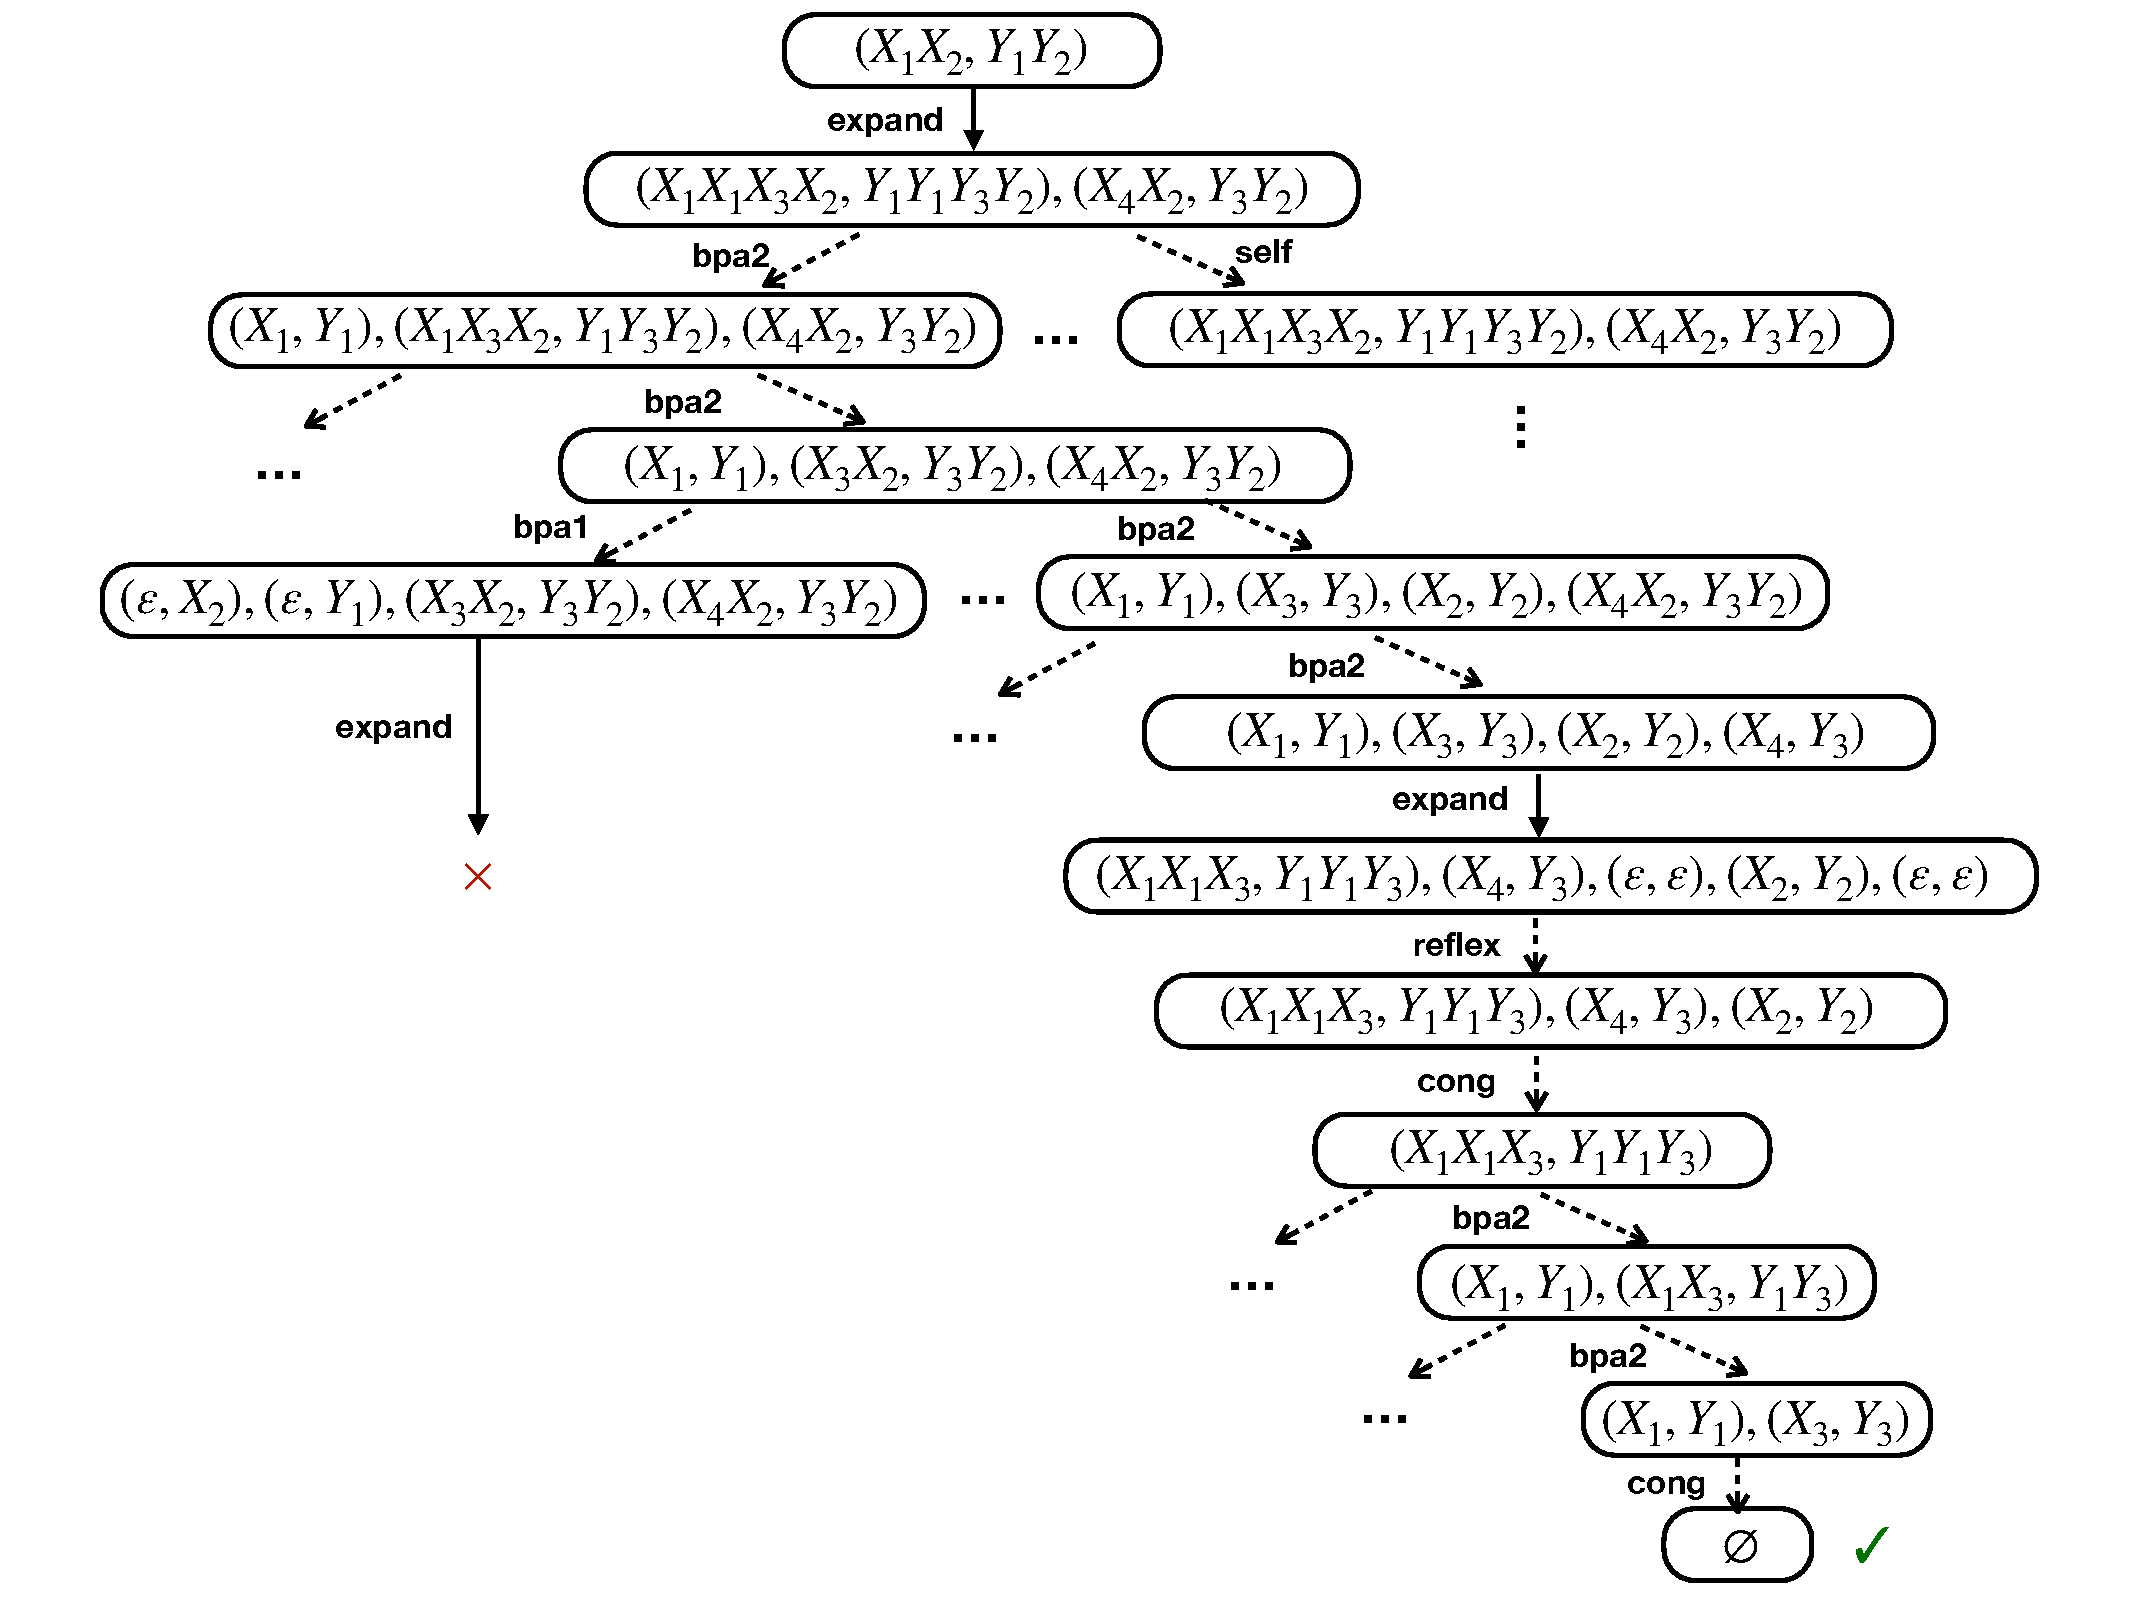
\includegraphics[width=12cm]{img/expansion_tree_example}  
  \caption{An example of an expansion tree}
  \label{fig:expansion-tree}
\end{figure}

\begin{example}
  The expansion tree for our running example is in
  Figure~\ref{fig:expansion-tree}. Once a successful branch is reached
  (depicted by the $\checkmark$ mark),
  $\Bisim(\vec X, \vec Y, \productions)$ returns $\True$.
\end{example}

\subsection{Checking the bisimilarity of context-free session types}

Function $\BisimT$ decides the equivalence of two well-formed and
renamed types, $S$ and $T$.  It starts by computing the start words
for $S$ and $T$ by first translating $S$ to a grammar and enriching
this with the productions for type $T$. After pruning the productions
in the grammar (function $\Prune$), the equivalence of $S$ and
$T$ is decided using function $\Bisim$.
%
\begin{align*}
  \BisimT(T, U) =&\ \Bisim(\vec X, \vec Y, \Prune (\productions))
  \\
  \mathsf{where}\ (\vec X, \productions') =&\ \grm (S, \emptyset)
  \\
  (\vec Y, \productions) =&\ \grm (T, \productions')
\end{align*}

%%% Local Variables:
%%% mode: latex
%%% TeX-master: "main"
%%% End:

\section{Correctness of the algorithm}
\label{sec:soundness}

In this section we prove that our algorithm is sound and complete
with respect to the meta-theory of context-free session types proposed
by Thiemann and Vasconcelos~\cite{thiemann2016context}.

We start by showing that the bisimulation relation on context-free
session types, $\TypeEquiv$, is equivalent to the bisimulation
relation obtained from the productions, $\ProdEquiv$.  Then, based on
results from Caucal~\cite{caucal1986decidabilite}, Christensen,
H{\"{u}}ttel, and Stirling~\cite{DBLP:journals/iandc/ChristensenHS95},
Jan{\v{c}}ar and Moller~\cite{janvcar1999techniques}, we conclude that
our algorithm is sound and complete.

\subsection{The two bisimulations coincide}

For the purpose of providing a bisimulation between context-free
session types and their corresponding symbols in the grammar, we start
with a lemma that relates terminated types~$S$ to the result of the
$\toGrammarf S$.

\begin{lemma}
  \label{lem:terminated-togrammar}
  %% replaced P by \emptyset
  \DONE S if and only if $\varepsilon, \emptyset = \toGrammarf S$.
\end{lemma}

\begin{proof} Given that all variables in a type are under some
  $\mu$-binder, there is a simple inductive characterization of
  $\DONE S$, namely, $\DONE \skipk$, $\DONE{(S;T)}$ if $\DONE S$ and
  $\DONE T$, $\DONE{(\mu X.S)}$ if $\DONE S$, $\DONE X$, and false in
  all other cases. The proof then follows by a simple induction on
  this characterization for the ``if'' direction, and induction on
  \lstinline|toGrammar| for the ``only if'' direction.
\end{proof}

To conclude that the bisimulations on context-free session types and
those on productions coincide, we present a bisimilarity between
context-free session types and the result of \lstinline|toGrammar|.
%
As the implementation of \isCheckedf is not shown, we assume that
$\isCheckedf S$ returns \lstinline|True| if and only if $\DONE S$.
%
%% new from here
Consider the relation $\mathcal{R}$ given by:
\[\begin{array}{lll}
	\mathcal{R} = & \{ (\skipk, (\varepsilon, \emptyset))\} \,\cup\\
	& \{(\sharp B,(X,\{X \rightarrow \sharp B\})) \mid \text{$B$ is any base type}\} 
	   \,\cup\\
	& \{ (\star\{l_i\colon S_i\}_{i\in I}, (X, \{X \rightarrow \star l_i
    \vec Y_i\}_{i\in I} \cup (\cup  P_i)_{i\in I})) \mid 
    \begin{array}[t]{l}
    	\text{$S_i$ is any type, $l_i$ is any label,}\\
    	\text{$Y_i, P_i = \toGrammarf{S_i}$, $i \in I$ }\} \,\cup\\
    \end{array}\\
    &\{(S_1;S_2, (\vec X_1\vec X_2,  P_1 \cup  P_2)) \mid
    \text{$S_i$ is any type, $\vec X_i, P_i = \toGrammarf{S_i}, i = 1,2$ } \}\,\cup\\
    & \{(\mu X.S, (\varepsilon, \emptyset)) \mid 
    \text{$S$ is any type with bounded variable $X$ and $\isCheckedf \mu X.S$}\}\,\cup\\
    & \{(\mu X.S, (X, \{X \rightarrow a \vec Z\vec Y\} \cup  P)) \mid 
    \begin{array}[t]{l}
      \text{$S$ is any type with bounded variable $X$, }\\
      \text{not }\isCheckedf \mu X.S, \\
      Y\vec Y, P = \toGrammarf{S} \text{ and } Y \rightarrow a \vec Z \in  P\}
    \end{array}\\
\end{array}\]

\begin{lemma}
\label{lemma:bisim_unr}
	For any type $S$, if not $\isCheckedf \mu X.S$ and 
	$(\mu X.S, (X, \{X \rightarrow a \vec Z\vec Y\} \cup  P))\in \mathcal{R}$
	with $Y \rightarrow a \vec Z \in  P$, then
	$(\Unravel(\mu X.S), (X, \{X \rightarrow a \vec Z\vec Y\} \cup  P))
	\in \mathcal{R}$.
\end{lemma}

\begin{proof}
	Notice that $Y \rightarrow a \vec Z \in  P$ is precisely the first 
	transition of $\Unravel(\mu X.S)$. Furthermore, since 
	$\subs{\mu X.S}{X} S$ is obtained from $S$ by 
	replacing the occurrences of $X$ by $\mu X.S$, all the productions for
	$\subs{\mu X.S}{X} S$ 
	are given by the productions of $S$, as using $\mu X.S$
	instead of $X$ does not contribute with any new production on $S$.
\end{proof}

\begin{lemma}
\label{lemma:bisim_semi}
	$(S_1;S_2, (\vec X_1\vec X_2,  P_1 \cup  P_2))\in\mathcal{R}$ iff 
	$(S_i, (\vec X_i,  P_i))\in\mathcal{R}$, for $i=1,2$.
\end{lemma}
\begin{proof}
	Assume that $(S_1;S_2, (\vec X_1\vec X_2,  P_1 \cup  P_2))\in\mathcal{R}$
	and $(S_i, (\vec Y_i,  Q_i))\in\mathcal{R}$. Since 
	$ \vec X_i, P_i = \toGrammarf{S_i}$ and, by construction of $\mathcal{R}$,
	we necessarily have $ \vec Y_i, Q_i = \toGrammarf{S_i}$, it follows that
	$\vec Y_i = \vec X_i$ and $Q_i=P_i$.
\end{proof}

With the same argument, we can prove the following lemma.

\begin{lemma}
\label{lemma:bisim_choice}
	$(\star\{l_i\colon S_i\}_{i\in I}, (X, \{X \rightarrow \star l_i
    \vec Y_i\}_{i\in I} \cup (\cup  P_i)_{i\in I}))\in\mathcal{R}$ iff 
	$(S_i, (\vec Y_i,  P_i))\in\mathcal{R}$, $i \in I$.
\end{lemma}

Now we prove that the relation $\mathcal{R}$ is a bisimilarity. We do it
by induction. For that, just notice that for any recursive type 
$\mu X.S$, $\Unravel(\mu X.S)$ is not a recursive type and preserves the 
transitions from $\mu X.S$.

\begin{theorem}
\label{thm:cfst_vs_grammar}
	$\mathcal{R}$ is a bisimilarity.
\end{theorem}

\begin{proof}
	We prove that for each $(S, (\vec X, P))\in \mathcal{R}$	, if
	$S \LTSderives[a] T$ then $\vec X \rightarrow a \vec Y\in P$
	and $(T, (\vec Y, P'))\in \mathcal{R}$ for some $P'$. The proof is by
	induction on the structure of $S$.
	\begin{itemize}
		\item $(\skipk, (\varepsilon, \emptyset))$: $\skipk$ does not have any
		transition.
		\item $(\sharp B,(X,\{X \rightarrow \sharp B\}))$: by the \LTS,
		$\sharp B\LTSderives[\sharp B] \skipk$ and $X\rightarrow \sharp B$ with
		$(\skipk, (\varepsilon, \emptyset))\in \mathcal{R}$.
		\item $(\star\{l_i\colon S_i\}_{i\in I}, (X, \{X \rightarrow \star l_i
    	\vec Y_i\}_{i\in I} \cup (\cup  P_i)_{i\in I}))$: 
    	$\star\{l_i\colon S_i\}_{i\in I}\LTSderives[l_i] S_i$ and 
    	$X \rightarrow \star l_i \vec Y_i$ for each $i\in I$. By 
    	lemma~\ref{lemma:bisim_choice}, $(S_i, (\vec Y_i,  P_i))\in\mathcal{R}$
    	for each $i\in I$. 
    	\item $(S_1;S_2, (\vec X_1\vec X_2,  P_1 \cup  P_2))$: start noting
    	that by lemma~\ref{lemma:bisim_semi} 
    	$(S_i, (\vec X_i, P_i))\in \mathcal{R}$, $i=1,2$.
    	\begin{itemize}
    	\item if 
    	$S_1;S_2\LTSderives[a] S_1'; S_2$ with $S_1\LTSderives[a] S_1'$, then 
    	$\Unravel(S_1)\LTSderives[a] S_1'$. By 
    	lemma~\ref{lemma:bisim_unr}, 
    	since $(S_1,(\vec X_1, P_1))\in\mathcal{R}$, we have
    	$(\Unravel(S_1), (\vec X_1, P_1))\in \mathcal{R}$ 
    	(if $S_1$ is not a recursive type, $\Unravel(S_1)$ 
    	coincides with $S_1$).
    	Hence, by induction hypothesis, we know that 
    	$\vec X_1 \rightarrow a \vec Y_1$ and 
    	$(S_1', (\vec Y_1,P_1'))\in \mathcal{R}$. 
    	By lemma~\ref{lemma:bisim_semi}, we conclude that 
    	$(S_1';S_2, (\vec Y_1 \vec X_2,P_1'\cup P_2))\in \mathcal{R}$. 
    	\item if $S_1;S_2\LTSderives[a] S_2'$, where $\DONE{S_1}$ and 
    	$S_2\LTSderives[a] S_2'$, it follows that 
    	$\Unravel(S_2)\LTSderives[a] S_2'$. Since
    	$(S_2, (\vec X_2, P_2))\in \mathcal{R}$ we have 
    	$(\Unravel(S_2), (\vec X_2, P_2))\in \mathcal{R}$. 
    	By induction hypothesis, we thus have
    	$\vec X_2 \rightarrow a \vec Y_2$ where 
    	$(S_2', (\vec Y_2,P_2'))\in \mathcal{R}$. Since $\DONE{S_1}$, by
    	lemma~\ref{lem:terminated-togrammar} $\vec X_1 = \varepsilon$, 
    	hence $\vec X_1 \vec X_2 = \vec X_2 \rightarrow a \vec Y_2$.
    	\end{itemize}
    	\item $(\mu X.S, (\varepsilon, \emptyset))$: in this case, 
    	$\isCheckedf \mu X.S$, thus
    	we do not have any transition (lemma~\ref{lem:terminated-togrammar}).
    	\item $(\mu X.S, (X, \{X \rightarrow a \vec Z\vec Y\} \cup  P))$: 
    	if $\mu X.S\LTSderives[l] T$, then $\Unravel(\mu X.S)\LTSderives[l] T$.
    	Furthermore, we know that 
    	$(\Unravel(\mu X.S), (X, \{X \rightarrow a \vec Z\vec Y\} \cup  P))
    	\in\mathcal{R}$. By induction hypothesis, it follows that $l=a$ and 
    	$(T, (\vec Z \vec Y, P'))\in \mathcal{R}$.
	\end{itemize} 
	The proof that any transition in the productions leads to a transition in 
	the corresponding type is very similar and is also done by induction. 
	For that,
	we only need to recall that the variable $X$ is a fresh variable and, thus, 
	the transitions from $X$ are simply the ones explicitly detailed in each 
	pair from $\mathcal{R}$.
\end{proof}


%% new until here

%% old proof here
%\begin{theorem}
%\label{thm:cfst_vs_grammar}
%  $S$ is bisimilar to $\toGrammarf{S}$.
%\end{theorem}
%
%\begin{proof}
%  Let $\mathcal R$ be the binary relation on types $\times$ (words
%  $\times$ productions) that contains the following sets of pairs
%  $(S, (\vec X, P))$ built in such a way that $\vec X, P = \toGrammarf S$.
%  %
%  \begin{gather*}
%    (\skipk, (\varepsilon, \emptyset))
%    \\
%    (\sharp B, (X, \{X \rightarrow \sharp B\}))
%    \\
%    (\star\{l_i\colon S_i\}_{i\in I}, (X, \{X \rightarrow \star l_i
%    \vec Y_i\}_{i\in I} \cup (\cup  P_i)_{i\in I}))
%    %
%    \text{ when } \vec Y_i, P_i = \toGrammarf{S_i}, i \in I
%    % \\
%    % (S_i, (\vec Y_i, \{X \LTSderivesP[\star l_i]
%    % \vec Y_i\}_{i\in I} \cup (\cup  P_i)_{i\in I}))
%    % %
%    % \text{ when } \vec Y_i, P_i = \toGrammarf{S_i}, i \in I
%    \\
%    (S_1;S_2, (\vec X_1\vec X_2,  P_1 \cup  P_2))
%    %
%    \text{ when } \vec X_i, P_i = \toGrammarf{S_i}, i = 1,2
%    % \\
%    % (S'_1;S_2, (\vec Y,  P_1 \cup  P_2))
%    % %
%    % \text{ and, in addition, } S_1 \LTSderives S_1' 
%    % \text{ and } \vec X_1\vec X_2 \rightarrow a \vec Y
%    % \\
%    % (S_2', (\vec Y,  P_1 \cup  P_2))
%    % %
%    % \text{ and, in addition, } \DONE{S_1}
%    % \text{ and } S_2 \LTSderives S_2' 
%    % \text{ and } \vec X_1\vec X_2 \rightarrow a \vec Y
%    \\
%    (\mu X.S, (\varepsilon, \emptyset))
%    \text{ when } \isCheckedf \mu X.S
%    \\
%    (\mu X.S, (X, \{X \rightarrow a \vec Z\vec Y\} \cup  P))
%    %
%    \text{ when not }  \isCheckedf \mu X.S \text{ and }
%    \\\quad
%    Y\vec Y, P = \toGrammarf{S}
%    \text{ and }
%    Y \rightarrow a \vec Z \in  P
%   %  \\
%   %  (T, (\vec Z\vec Y, \{X \LTSderivesP \vec Z\vec Y\} \cup  P))
%   %  %
%   %  \text{ and, in addition, } Y \LTSderivesP \vec Z
%   % \text{ and } \subs{\mu X.S}{X} S \LTSderives T
%  \end{gather*}
%  %
%  That $\mathcal R$ is a bisimulation follows by co-induction, using
%  Lemma~\ref{lem:terminated-togrammar}. % and the fact that
%  % $S \bisim \subs{\mu X.S}{X} S$~\cite{thiemann2016context}.
%\end{proof}

% We start by showing that the initial (dummy) production does not
% affect bisimulation checking.
% %
% \begin{lemma}
%   \label{lem:dummy}
%   $X_S \ProdEquiv X_T$ if and only if
%   $\toGrammarf S \ProdEquiv \toGrammarf T$.
% \end{lemma}

% \begin{proof}
%   We have $X_S \rightarrow\, \initialProd\,(\toGrammarf S)$ and
%   $X_T \rightarrow\, \initialProd\,(\toGrammarf T)$.
%   Hence, $X_S \TypeEquiv X_T$ if and only if
%   $\toGrammarf S \ProdEquiv \toGrammarf T$. \vv{prove both directions separately}
% \end{proof}

% Terminated session types do not originate new productions.

% \begin{lemma}
%   \label{lemma:terminated_session}
%   If \DONE{S}, then \upshape{\lstinline|toGrammar |}$S$ adds no
%   productions and returns \upshape{\lstinline|[]|}.
% \end{lemma}

% \begin{itemizeproof}
%   By rule induction  on the hypothesis.
%   \begin{itemize}
%   \item If $S\triangleq \skipk$, then \lstinline{toGrammar} adds no
%     productions and returns \lstinline{[]}.
%   \item If $S\triangleq S;T$, then \DONE S and \DONE T. By induction,
%     the recursive calls add no productions and return
%     \lstinline|[]|. Then, function \lstinline|toGrammar| returns
%     \lstinline|[]++[]|, which evaluates to \lstinline|[]|.
%   \item If $S\triangleq \mu X. T$, then
%     $\subs{S}{X}T \checkmark$.
%     %
%     Function \lstinline|toGrammar |$S$ adds the productions from
%     \lstinline|toGrammar (subs (Var y) X t)|. But $\subs{S}{X} T$ is a
%     terminated session, thus \lstinline{toGrammar }$T$ adds no
%     productions and returns \lstinline{[]}. \vv{co-induction?}.
%   \end{itemize}
% \end{itemizeproof}

% Now we prove that any transition in the \LTS\ has a
% corresponding transition derived from the set of productions.

% \begin{lemma}
%   \label{lem:type-to-prod}
%   If $S \LTSderives T$, then \upshape{\lstinline|toGrammar|}
%   $S \LTSderivesP \vec X$ and \upshape{\lstinline|toGrammar|} $T$ is a
%   prefix of~$\vec X$.
% \end{lemma}

% \begin{itemizeproof}
% By rule induction on the hypothesis.
% \begin{itemize}
% \item If $S\triangleq \sharp B$, then
%   $S \LTSderives[\sharp B] \skipk$. The call $\toGrammarf S$
%   returns a fresh variable $Y$ and inserts a production
%   $Y\rightarrow \sharp B$. Then $S \LTSderivesP \varepsilon$ and
%   $\toGrammarf\,\skipk =$ \lstinline{[]}, that is, $\varepsilon$.
% \item If $S\triangleq \star\{l_i``\colon S_i\}_{i\in I}$ then,
%   $S \LTSderives[\star l_j] S_j$, for each $j\in I$. Function
%   $\toGrammarf S$ returns a fresh variable $Y$ and, recursively,
%   inserts a production $Y\rightarrow \star l_j (\toGrammarf{S_j})$,
%   for each $j\in I$, hence
%   $Y \LTSderivesP[\star l_j] \toGrammarf{S_j}$.
% \item If $S\triangleq T;U$ and $T \LTSderives[a] T'$, then
%   $S \LTSderives[a] T';U$.  By induction hypothesis, $\toGrammarf T$
%   adds the production $Y\rightarrow a (\toGrammarf{T'})$, where $Y$
%   is a fresh variable.  We notice that $\toGrammarf T$
%   $= Y \vec Y_T$ for some sequence of non-terminal symbols
%   $\vec Y_T$. By congruence, we have:
%   \[\toGrammarf S = Y\vec Y_T(\toGrammarf U)
%     \rightarrow a(\toGrammarf T')\vec Y_T(\toGrammarf U)
%     .\]
% \item If $S\triangleq \mu x.T$, then $\subs SXT \LTSderives T'$.
%   By induction, the corresponding production in
%   %
%   \lstinline{toGrammar (subs (Var y) x t)} is recursively added by
%   $\toGrammarf S$ in the form $Y \rightarrow a (\toGrammarf{T'})$,
%   where $Y$ is a fresh variable that is, then, returned by
%   $\toGrammarf S$.
% \item If $S\triangleq T;U$, $T$ is a terminated session, with no further
%   action, and $U \LTSderives[a] U'$ then, using the \LTS\ we have
%   $T;U \LTSderives[a] U'$. On the other hand, by induction hypothesis and
%   using Lemma~\ref{lemma:terminated_session}:
%   \begin{itemize}
%   \item $\toGrammarf T$  returns \lstinline{[]},
%   \item $\toGrammarf U$ adds a production
%     $Y \rightarrow a (\toGrammarf U')$, where $Y$ is a fresh
%     variable.
%   \end{itemize}
%   We notice that $\toGrammarf U = Y\vec Y_U$ for some sequence of
%   non-terminal symbols $\vec Y_U$. Hence, by congruence, we have a
%   transition
%   \[\toGrammarf S = \text{\lstinline{[]}} Y
%     \vec Y_U \rightarrow a (\toGrammarf{U')} \vec Y_U.\]
% \end{itemize}
% \end{itemizeproof}

% Conversely, we prove that any transition derived from the productions
% has a corresponding labelled transition in the \LTS.

% \begin{lemma}
%   \label{lem:prod-to-type}
%   If $\toGrammarf S \LTSderivesP \vec Y$, then $S\LTSderives
%   T$.\\ \vv{and there must be some relation on $\vec Y$ and $T$, for
%     induction purposes}
% \end{lemma}

% \begin{itemizeproof}
%   By induction on the structure of $S$: \vv{redo}
%   \begin{itemize}
%   \item If $S \triangleq \sharp B$, then $\toGrammarf S$ adds the
%     production $Y\rightarrow \sharp B$ and we know that
%     $S \LTSderivesP[\sharp B] \skipk$.
%   \item If $S\triangleq \star \{\ell_i : S_i\}_{i\in I}$, then
%     $\toGrammarf S$ recursively adds
%     $\toGrammarf S \rightarrow \star \ell_j(\toGrammarf{Sj})$ for each
%     $j\in I$. In the \LTS\ for productions we also have
%     $S \LTSderivesP[\star\ell_j] S_j$ for each $j\in I$.
%   \item If $S \triangleq T;U$, then $\toGrammarf S$ recursively adds
%     all productions from $\toGrammarf T$ and from $\toGrammarf
%     U$. Hence, if $\toGrammarf S \LTSderivesP \vec Y$ then, either:
%     \begin{itemize}
%     \item $\toGrammarf T \LTSderivesP \vec Y$ and, in this case, by
%       induction we know that $T \LTSderives T'$ and from the \LTS\ for
%       productions we obtain $S \LTSderivesP T';U$;
%     \item \DONE{T} and $\toGrammarf U \rightarrow a\vec Y$ and, by
%       induction we know that $U \LTSderives[a] U'$ and from the \LTS\
%       for productions we obtain $S \LTSderives U'$.
%     \end{itemize}
%   \item If $S\triangleq \mu x.T$, then $\toGrammarf S$ adds,
%     recursively, all productions from
%     %
%     \lstinline|toGrammar (subs (Var y) x t)|.  Analogously, in the
%     \LTS\ for productions, any transition $\subs SXT \LTSderives T'$
%     leads to a transition $S \LTSderives T'$. \vv{Why?}
%   \end{itemize}
% \end{itemizeproof}

% Having proved that any labelled transition in the LTS has a corresponding
% transition in the grammar and vice-versa, the following theorem is now
% immediate.

% \begin{theorem}
%   \label{thm:cfst_vs_grammar}
%   $S\TypeEquiv T$  if and only if $ X_S \ProdEquiv X_T$.
% \end{theorem}

% \begin{proof}
%   From lemmas~\ref{lem:dummy}, \ref{lem:type-to-prod}, and~\ref{lem:prod-to-type}.
% \end{proof}

% \subsection{Unnormedness is preserved by pruning} % Not needed?

% To prove that the pruning stage is in accordance with the results from
% Christensen et al.~\cite{DBLP:journals/iandc/ChristensenHS95}, we
% observe that unnormed non-terminal symbols corresponding to (un)normed
% types are (un)normed. These results follow immediately from the
% previous results. \vv{from which results, exactly?}

% \begin{corollary}
%   Given a context-free session type $S$, $|S| = |\toGrammarf S|$.
% \end{corollary}

% \begin{corollary}
%   A context-free session type $S$ is unnormed if and only if $X_S$ is
%   unnormed.
% \end{corollary}

% \vv{these notions are not defined on session types}

\subsection{Correctness of the algorithm}

We now focus on the correctness of the algorithm in
Listing~\ref{lst:algorithm}.  Before proceeding to soundness, we
recall the \emph{safeness property} presented by Jan{\v{c}}ar and
Moller.

\begin{proposition} [Safeness Property \cite{janvcar1999techniques}]
  \label{prop:safeness}
  $\vec X \ProdEquiv \vec Y$ if and only if the expansion tree rooted
  at $\{(\vec X, \vec Y)\}$ has a successful branch.
\end{proposition}

Notice that function \lstinline|bisimilar|
(Listing~\ref{lst:algorithm}) builds an expansion tree by alternating
between expansion and simplification operations (reflexive,
congruence and \BPA\ rules), as proposed by Jan{\v{c}}ar and Moller.
%
These simplification rules are \emph{safe}~\cite{janvcar1999techniques}, in the sense that the
application of any rule preserves the bisimulation from a parent node
to at least one child node and, reciprocally, that bisimulation on a
child node implies the bisimulation of its parent node, thus proving
the safeness property.

%\begin{proof}
%	On the other hand, as observed in~\cite{janvcar1999techniques},
%	the union of nodes along a successful branch is a relation $R$
%	such that $R\subseteq \ProdEquiv$. Hence, any pair $(\vec X, \vec Y)$
%	occurring along a successful branch is such that $\vec X \ProdEquiv \vec Y$,
%	which, by Lemma~\ref{lemma:filtering}, means that $|\vec X|=|\vec Y|$.
%	So, the filtering rule would node exclude any node in the successful branch
%	and, then, also preserved the safeness property.
%\end{proof}

\begin{lemma}
  \label{lem:bisimilar-to-prod}
  If $\bisimf S T$ returns \upshape{\lstinline|True|}, then
  $X_{S} \ProdEquiv X_{T}$.
	% Given two context-free session types $S$ and $T$, if the function
	% \lstinline|equivalent|, presented in Listing~\ref{lst:algorithm},
	% returns \lstinline|true|, then $X_{S} \ProdEquiv X_{T}$.
\end{lemma}

\begin{proof}
  Function \lstinline|bisimilar| returns \lstinline|True| for $S$ and
  $T$ whenever it reaches a (finite) successful branch in the expansion
  tree rooted at $\{(X_{S}, X_{T})\}$. Conclude with the safeness property,
  Proposition~\ref{prop:safeness}.
  % , whenever the expansion tree rooted
  % at $\{(X_{S}, X_{T})\}$ has a (finite) successful branch, we
  % kn that $X_{S} \ProdEquiv X_{T}$.
\end{proof}

From the previous results, the soundness of our algorithm is now
immediate: the algorithm to check the bisimulation of context-free
session types (Listing~\ref{lst:algorithm}) is sound with respect to
the meta-theory of context-free session types.

\begin{theorem}
  If $\bisimf ST$ returns \upshape{\lstinline|True|} then $S\TypeEquiv T$.
\end{theorem}

\begin{proof}
  From Theorem~\ref{thm:cfst_vs_grammar} and
  Lemma~\ref{lem:bisimilar-to-prod}.
\end{proof}

Having observed that the safeness property was paramount for
soundness, we now notice that the \emph{finite witness property} is of
utmost importance to prove completeness. This result follows
immediately from the analysis by Jan{\v{c}}ar and
Moller~\cite{janvcar1999techniques}, which capitalizes on results by
Caucal~\cite{caucal1986decidabilite}, and Christensen, H{\"{u}}ttel, and
Stirling~\cite{DBLP:journals/iandc/ChristensenHS95}:

\begin{proposition} [Finite Witness Property]
\label{finite_witness}
	If $\vec X \ProdEquiv \vec Y$, then the expansion tree rooted at
	$\{(\vec X, \vec Y)\}$ has a finite successful branch.
\end{proposition}

We refer to Caucal, Christensen, H{\"{u}}ttel, and Stirling for
details on the proof of existence of a finite witness, as stated in
Proposition~\ref{finite_witness}. This proof is particularly
interesting in that it highlights the importance of BPA rules and of
pruning productions on reaching such (finite) witness. The results in
these two papers also allow us to unravel the reason for the
distinction of the simplification phase in the case where all the
symbols in the grammar are normed from the case where they are not, as
presented in Listing~\ref{lst:algorithm}.

Proposition~\ref{finite_witness} paved the way to obtain the completeness result. 
We now prove that the algorithm to check the bisimulation of context-free session 
types is complete with respect to the meta-theory of context-free session
types.

\begin{theorem}
  If $S \TypeEquiv T$ then $\bisimf S T$ returns
  \upshape{\lstinline|True|}.
\end{theorem}

\begin{proof}
  Assuming that $S \TypeEquiv T$, by Theorem~\ref{thm:cfst_vs_grammar}
  we have $X_{S} \ProdEquiv X_{T}$.  Hence, the Proposition~\ref{finite_witness}
  ensures the existence of a finite successful branch on the
  expansion tree rooted at $\{(X_{S},X_{T})\}$, i.e., a branch
  terminating in an empty node.  Since our algorithm traverses the
  expansion tree using breadth-first search it will, eventually, reach
  the empty node and conclude the bisimulation positively.
\end{proof}

%%% Local Variables:
%%% mode: latex
%%% TeX-master: "main"
%%% End:

\section{Optimizations}
\label{sec:optimisations}

Armed with the results in Section~\ref{sec:algorithm}, we decided to
benchmark the algorithm on a test suite of carefully crafted pair of
types (more on this in Section~\ref{sec:evaluation}). During this 
process we came across a pair of types,
\begin{equation}
\label{ex:chaotic}
\begin{aligned}
  S &\triangleq \mu x . \&\{ \mathsf{Add}\colon x;x; !\,\intk,
  \mathsf{Const}\colon ?\,\intk;!\intk,
  \mathsf{Mult}\colon x;x;!\,\intk\}
  \\
  T &\triangleq \mu x . \&\{ \mathsf{Add}\colon x;x,
  \mathsf{Const}\colon ?\,\intk,
  \mathsf{Mult}\colon x;x\}; !\,\intk
\end{aligned}
\end{equation}
%
on which function \lstinline|bisimilar| took 4379.98 seconds (that is
one hour and forty minutes) to terminate. This is certainly not a
reasonable running time for an algorithm to be included in a
compiler. Hence we looked into ways to improve the running time. Among
the different optimisations that we tried, two stand out:
\begin{enumerate}
\item Iterate the simplification stage until a fixed point is reached;
\item Use a double-ended queue where promising children are prepended
  rather than appended.
\end{enumerate}

If, on the one hand, we believed that the computation of the expansion
tree could be speeded up by extending the simplification phase, on the
other hand we suspected that a double-ended queue would allow
prioritizing nodes with potential to reach an empty node faster.
%
Iterating the simplification procedure on a given node $N$, the
algorithm computes the simplest possible children nodes derived from
$N$. Of course, we need to make sure that a fixed-point exists, which
we do with Theorem~\ref{thm:fixed_point}.
%
Using a double-ended queue, the algorithm prepends (rather than
appends) nodes that are already empty or whose pairs $(\vec X, \vec Y)$
are such that $|\vec X|\leq 1$ and $|\vec Y| \leq 1$.
%
The revised \lstinline|simplify| function is in Listing~\ref
{lst:enhanced}.

The next theorem shows that the simplification function that consists
in applying the reflexive, congruence and \BPA\ rules has a fixed
point.  The result applies regardless of whether all nonterminal
symbols symbols are normed or not.

\begin{theorem}
  \label{thm:fixed_point}
  The simplification function that results from applying the
  reflexive, congruence, and \BPA\ rules, has a fixed point in the
  complete partial ordered set
  {\upshape\lstinline|Set (Node, Ancestors)|}, where the set of
  ancestors is supposed to be fixed. % and equal to $A$.
\end{theorem}

\begin{proof}
  Throughout the proof we abuse notation and denote the application
  of simplification rules to nodes and to elements of
  $\text{\lstinline{Set (Node, Ancestors)}}$ similarly, when no
  ambiguity arises.
%
  Consider the order $\leqSets$, defined on
  $\text{\lstinline{Set (Node, Ancestors)}} \times
  \text{\lstinline{Set (Node, Ancestors)}}$, as $S_1 \leqSets S_2$ if
  $|S_1| \leq |S_2|$ and there exists an injective map
  $\sigma : S_1 \rightarrow S_2$ s.t.\ $\sigma(N_1,A) = (N_2,A)$ with
  $N_2\subseteq N_1$.
  % 
  \begin{itemize}
  \item $\leqSets$ is a partial order. The proof that $\leqSets$ is
    reflexive and transitive is straightforward.  To prove that it is
    antisymmetric, assume that $S_1\leqSets S_2$ and
    $S_2 \leqSets S_1$.  This means that $|S_1|=|S_2|$ and,
    furthermore, the maps $\sigma_1 : S_1 \rightarrow S_2$ and
    $\sigma_2 : S_2 \rightarrow S_1$ are bijective. Notice that
    $\sigma_1\circ \sigma_2$ is the identity map, otherwise we could
    consider $(N,A)\in S_2$ where $N$ is minimal w.r.t.\ inclusion and
    s.t.\ $(\sigma_1\circ \sigma_2)(N,A) \neq (N,A)$, i.e.,
    $(\sigma_1\circ \sigma_2)(N,A) = (N',A)$ with $N'\subseteq N$ for
    some $(N',A)\in S_2$; due to the minimality of $N$, we would have
    $(\sigma_1\circ \sigma_2)(N',A) = (N',A)$, which would contradict
    the injectivity of $\sigma_1\circ \sigma_2$. Since
    $\sigma_1 (N,A) = (N',A)$ is such that $N'\subseteq N$, we shall
    have $\sigma_1 (N,A) = (N,A)$. Hence, $S_1=S_2$.
  \item The simplification function is order-preserving.
	To prove that the reflexive rule preserves the order, let
        $S_1$ and $S_2$ be s.t.\ $S_1\leqSets S_2$ and let us prove
        that
        $\text{\lstinline{reflex}}
        S_1\leqSets\text{\lstinline{reflex}}S_2$.
	% Start noticing that $|S| = |\text{\lstinline{reflex}} S|$,
	% hence
	% the number of children nodes is preserved by using the
	% reflexive
	% rule, let us analyze each case.
	Let $(N,A)\in \text{\lstinline{reflex}} S_1$ and notice that
        there exists $(N_1,A)\in S_1$, such that
        $\text{\lstinline{reflex}} N_1 = N $, and so, in $S_2$ there
        is $(N_2,A)=\sigma(N_1,A)$ s.t. $N_2\subseteq N_1$.  Since
        $N_2\subseteq N_1$, we have
        $\text{\lstinline{reflex}} N_2 \subseteq
        \text{\lstinline{reflex}} N_1 = N$.  The same reasoning
        applies to prove that if $S_1\leqSets S_2$ then
        $\text{\lstinline{congruence} }
        S_1\leqSets\text{\lstinline{congruence} }S_2$.
%
	To prove that \lstinline{bpa1} preserves the order,
	note that 
	$S \subseteq \text{\lstinline{bpa1} }S$. Assume that 
	$S_1\leqSets S_2$, let $(N,A)\in \text{\lstinline{bpa1} }S_1$, 
	and denote by $(N_1,A)\in S_1$ and $(\vec X,\vec Y)\in N_1$  
	the node and the pair whose simplification 
	led to $(N,A)$. We know that exists $(N_2,A)\in S_2$
	s.t.\ $N_2 \subseteq N_1$. If $(\vec X,\vec Y)\in N_2$,
	then the \lstinline{bpa1} simplification of $N_2$ with
	the pair $(\vec X,\vec Y)$ generates 
	$(N',A)\in \text{\lstinline{bpa1} }S_2$ such that 
	$N'\subseteq N$. On the other hand, if 
	$(\vec X,\vec Y)\not \in N_2$, then $N_2\subseteq N$ 
	and, since  $S_2 \subseteq \text{\lstinline{bpa1} }S_2$,
	$(N_2,A)\in \text{\lstinline{bpa1} }S_2$ is such that
	$N_2\subseteq N$.
	The same reasoning applies to \lstinline{bpa2}. 
      \end{itemize}
      
      Having proved that each simplification function preserves the
      order, and since the simplification procedure results from the
      successive application of these rules, we have proved that the
      simplification function also preserves the order.\smallskip
      %
      \begin{itemize}
      \item $(\text{\lstinline{Set (Node, Ancestors)}}, \leqSets)$ is
        a lattice. Given
        $S_1, S_2\in \text{\lstinline{Set (Node, Ancestors)}}$,
        $S_1 \cup S_2$ is an upper bound and $S_1 \cap S_2$ is a lower
        bound for $S_1$ and $S_2$.
      \item $(\text{\lstinline{Set (Node, Ancestors)}}, \leqSets)$ is
        a complete lattice. Given
      $\mathcal{B}\subseteq \text{\lstinline{Set (Node, Ancestors)}}$:
      $\bigcup_{S\in \mathcal{B}} S$ is an upper bound and
      $\bigcap_{S\in \mathcal{B}} S$ is a lower bound for the sets in
      $\mathcal{B}$.
    \end{itemize}
    Using Tarski's fixed point theorem~\cite{tarski1955lattice}, we
    conclude that the simplification function has a fixed point in
    $\text{\lstinline{Set (Node, Ancestors)}}$.
\end{proof}

Having proved that the fixed point exists, we can now adapt the
simplification phase to, on the one hand, iterate the simplification
rules until reaching a fixed point and, on the other hand, identify
and prepend promising nodes. An improved version of the
\lstinline|simplify| function (Listing~\ref{lst:algorithm}) is in
Listing~\ref{lst:enhanced}.

\begin{lstlisting}[
  caption={Haskell code for the improved simplification step (replaces
    function \lstinline|simplify| in Listing~\ref{lst:algorithm})},
  label={lst:enhanced},
  captionpos=b]
simplify :: Productions -> Node -> Ancestors -> NodeQueue -> NodeQueue
simplify ps n a q = foldr enqueueNode (Queue.dequeue q) nas
  where nas = findFixedPoint ps (Set.singleton (n,a))

enqueueNode :: (Node,Ancestors) -> NodeQueue -> NodeQueue
enqueueNode (n,a) q
 | maxLength n <= 1 = Queue.prepend (n,a) q
 | otherwise        = Queue.append (n,a) q

findFixedPoint :: Productions -> Set.Set (Node,Ancestors) -> 
                    Set.Set (Node,Ancestors)
findFixedPoint ps nas
  | nas == nas' = nas
  | otherwise   = findFixedPoint ps nas'
  where nas' = if allNormed ps
               then foldr (apply ps) nas [reflex,congruence,bpa2]
               else foldr (apply ps) nas [reflex,congruence,bpa1,bpa2]
\end{lstlisting}

The optimisations we propose aim at improving the performance of the
algorithm, however the branching nature of the expansion tree promotes
an exponential complexity: each simplification step (potentially)
generates a polynomial number of nodes, each of which with linear size
on the size of the input.  In turn, the same simplification phase may,
in the worst case, be iterated a linear number of times on the size of
the input.  For these reasons the complexity turns out to be (at least)
exponential.  Nevertheless, these heuristics seem to work quite well
in practice, as we show in the next section.

%%% Local Variables:
%%% mode: latex
%%% TeX-master: "main"
%%% End:

\section{Evaluation}
\label{sec:evaluation}

% \vv{estes testes incluem o tempo de parsing? nao deveriam. deveriam só
%   contar o tempo da chamada à funcao bisimilar/equivalent.}

We implemented the algorithm sketched in Listings~\ref{lst:toGrammar}
to~\ref{lst:enhanced} in 300 lines of Haskell and used the Glasgow
Haskell Compiler, GHC version 8.6.3, from which we have obtained the
results we present in this section.  Evaluation was conducted on a Mac
mini equipped with a 3.6 GHz Intel Core i3, 8 GB of memory, running
MacOS 10.14.3.

Once the improvement proposals were established, we benchmarked the
algorithm on a test suite of carefully crafted pair of types. These
tests comprise valid and invalid equivalences, for a total of 138
tests. We have profiled our program for the time and memory allocated
during the tests. For this purpose, we have used GHC's profiling
feature, that maintains a cost-centre stack to keep track of the
incurred costs. We ran the tests 10 times, kept a record of the run
time and memory allocated for each run, discarded the best and worst
values obtained and, then, we have measured the average of the
remaining values. The results are depicted in
Figure~\ref{fig:results}.

\begin{figure}[h]
	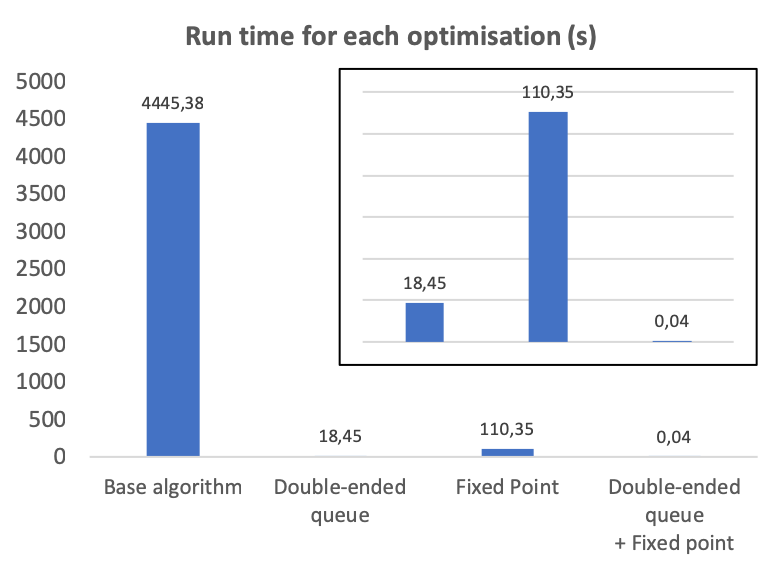
\includegraphics[height=5cm]{img/run_time}	\enspace
	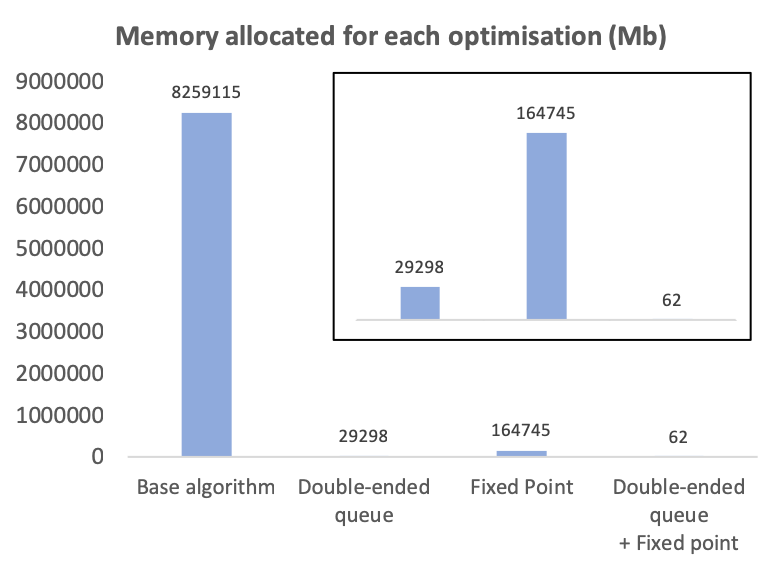
\includegraphics[height=5cm]{img/memory_alloc}
	\caption{Test results: running times (on the left) and
	memory allocated (on the right) checking the equivalence
	of context-free session types in 138 tests.}
	\label{fig:results}
\end{figure}

For the base algorithm, proposed in Listing~\ref{lst:algorithm}, we
obtained an average running time of about 4445.38 seconds and
8,259,115 Mb memory allocated. From the moment we introduced the
optimizations the results improved remarkably: iterating the
simplification phase in the search for a fixed point allowed to reduce
the running time to 110.35 seconds and the memory allocated to 164,745
Mb, whereas the implementation of the double-ended queue allowed to
reduce the running time to 18.45 seconds and the allocated memory to
29,298. The combination of both exhibit an improvement on more than
11,000,000\% from the base case, achieving an average of 0.04
seconds for the running time and 62 Mb of allocated memory.

We should also highlight that, we run example~\eqref{ex:chaotic}
with the improved algorithm, in a battery of 100 runs, and obtained an
average running time of 0.008 seconds.

The heuristic we proposed actually circumvents the exponential complexity 
inherent to the expansion tree, thus allowing to obtain running times that 
are manifestly small, thus allowing the use of this algorithm as an integral 
part of a compiler, as we had intended from the beginning.

%%% Local Variables:
%%% mode: latex
%%% TeX-master: "main"
%%% End:

\section{The bright future of \freest{}}
\label{sec:conclusion}

We have developed a basic compiler for \freest, a concurrent
functional programming with context-free session types, based on the
ideas of Thiemann and Vasconcelos~\cite{DBLP:conf/icfp/ThiemannV16}.
%
There are many possible extensions to the language. We discuss a
few. Shared channels allow for multiple readers and multiple writers,
thus introducing (benign) races. There are several proposals in the
literature~\cite{DBLP:journals/pacmpl/BalzerP17,
  DBLP:conf/sefm/FrancoV13,Lindley.Morris_Lightweight.functional.session.types,DBLP:journals/iandc/Vasconcelos12}
on which we may base this extension.
%
Because \freest{} compiles to Haskell, a better interoperability is
called for. We plan to add primitive support for lists, and for some
functions in Haskell's prelude, rank-1 functions that do not collide
with linearity constraints.
%
We have chosen a synchronous semantics for the communication
primitives, but we plan to experiment with buffered channels by simply
replacing the back-end.
%
The original proposal of context-free sessions is based on a
call-by-value operational semantics and we kept that strategy in
\freest. We however plan to experiment with call-by-need, taking
advantage of the back-end in Haskell. We also intend to allow messages
and choices to contain any functional or session type, rather than
containing only basic types. To achieve this,
the type equivalence algorithm for context-free session 
types should be intertwined with the type equivalence
algorithm for functional types, which is a challenging task.
Finally, we plan to incorporate type inference on type 
applications in order to allow the automatic identification of the
unifier matching a polymorphic type with the next type.

%%% Local Variables:
%%% mode: latex
%%% TeX-master: "main"
%%% End:


%\label{sect:bib}
\bibliographystyle{plain}
%\bibliographystyle{plainurl}
\bibliography{biblio}

%\section{Additional proofs}
\label{sec:additional-proofs}

\begin{proof}[Proof of Theorem~\ref{thm:fixed_point}]
  Throughout the proof we abuse notation and denote the application
  of simplification rules to nodes and to elements of
  $\text{\lstinline{Set (Node, Ancestors)}}$ similarly, when no
  ambiguity arises.
%
  Consider the order $\leqSets$, defined on
  $\text{\lstinline{Set (Node, Ancestors)}} \times
  \text{\lstinline{Set (Node, Ancestors)}}$, as $S_1 \leqSets S_2$ if
  $|S_1| \leq |S_2|$ and there exists an injective map
  $\sigma : S_1 \rightarrow S_2$ s.t.\ $\sigma(N_1,A) = (N_2,A)$ with
  $N_2\subseteq N_1$.
  % 
  \begin{itemize}
  \item $\leqSets$ is a partial order. The proof that $\leqSets$ is
    reflexive and transitive is straightforward.  To prove that it is
    antisymmetric, assume that $S_1\leqSets S_2$ and
    $S_2 \leqSets S_1$.  This means that $|S_1|=|S_2|$ and,
    furthermore, the maps $\sigma_1 : S_1 \rightarrow S_2$ and
    $\sigma_2 : S_2 \rightarrow S_1$ are bijective. Notice that
    $\sigma_1\circ \sigma_2$ is the identity map, otherwise we could
    consider $(N,A)\in S_2$ where $N$ is minimal w.r.t.\ inclusion and
    s.t.\ $(\sigma_1\circ \sigma_2)(N,A) \neq (N,A)$, i.e.,
    $(\sigma_1\circ \sigma_2)(N,A) = (N',A)$ with $N'\subseteq N$ for
    some $(N',A)\in S_2$; due to the minimality of $N$, we would have
    $(\sigma_1\circ \sigma_2)(N',A) = (N',A)$, which would contradict
    the injectivity of $\sigma_1\circ \sigma_2$. Since
    $\sigma_1 (N,A) = (N',A)$ is such that $N'\subseteq N$, we shall
    have $\sigma_1 (N,A) = (N,A)$. Hence, $S_1=S_2$.
  \item The simplification function is order-preserving.
	To prove that the reflexive rule preserves the order, let
        $S_1$ and $S_2$ be s.t.\ $S_1\leqSets S_2$ and let us prove
        that
        $\text{\lstinline{reflex}}
        S_1\leqSets\text{\lstinline{reflex}}S_2$.
	% Start noticing that $|S| = |\text{\lstinline{reflex}} S|$,
	% hence
	% the number of children nodes is preserved by using the
	% reflexive
	% rule, let us analyze each case.
	Let $(N,A)\in \text{\lstinline{reflex}} S_1$ and notice that
        there exists $(N_1,A)\in S_1$, such that
        $\text{\lstinline{reflex}} N_1 = N $, and so, in $S_2$ there
        is $(N_2,A)=\sigma(N_1,A)$ s.t. $N_2\subseteq N_1$.  Since
        $N_2\subseteq N_1$, we have
        $\text{\lstinline{reflex}} N_2 \subseteq
        \text{\lstinline{reflex}} N_1 = N$.  The same reasoning
        applies to prove that if $S_1\leqSets S_2$ then
        $\text{\lstinline{congruence} }
        S_1\leqSets\text{\lstinline{congruence} }S_2$.
%
	To prove that \lstinline{bpa1} preserves the order,
	note that 
	$S \subseteq \text{\lstinline{bpa1} }S$. Assume that 
	$S_1\leqSets S_2$, let $(N,A)\in \text{\lstinline{bpa1} }S_1$, 
	and denote by $(N_1,A)\in S_1$ and $(\vec X,\vec Y)\in N_1$  
	the node and the pair whose simplification 
	led to $(N,A)$. We know that exists $(N_2,A)\in S_2$
	s.t.\ $N_2 \subseteq N_1$. If $(\vec X,\vec Y)\in N_2$,
	then the \lstinline{bpa1} simplification of $N_2$ with
	the pair $(\vec X,\vec Y)$ generates 
	$(N',A)\in \text{\lstinline{bpa1} }S_2$ such that 
	$N'\subseteq N$. On the other hand, if 
	$(\vec X,\vec Y)\not \in N_2$, then $N_2\subseteq N$ 
	and, since  $S_2 \subseteq \text{\lstinline{bpa1} }S_2$,
	$(N_2,A)\in \text{\lstinline{bpa1} }S_2$ is such that
	$N_2\subseteq N$.
	The same reasoning applies to \lstinline{bpa2}. 
      \end{itemize}
      
      Having proved that each simplification function preserves the
      order, and since the simplification procedure results from the
      successive application of these rules, we have proved that the
      simplification function also preserves the order.\smallskip
      %
      \begin{itemize}
      \item $(\text{\lstinline{Set (Node, Ancestors)}}, \leqSets)$ is
        a lattice. Given
        $S_1, S_2\in \text{\lstinline{Set (Node, Ancestors)}}$,
        $S_1 \cup S_2$ is an upper bound and $S_1 \cap S_2$ is a lower
        bound for $S_1$ and $S_2$.
      \item $(\text{\lstinline{Set (Node, Ancestors)}}, \leqSets)$ is
        a complete lattice. Given
      $\mathcal{B}\subseteq \text{\lstinline{Set (Node, Ancestors)}}$:
      $\bigcup_{S\in \mathcal{B}} S$ is an upper bound and
      $\bigcap_{S\in \mathcal{B}} S$ is a lower bound for the sets in
      $\mathcal{B}$.
    \end{itemize}
    Using Tarski's fixed point theorem~\cite{tarski1955lattice}, we
    conclude that the simplification function has a fixed point in
    $\text{\lstinline{Set (Node, Ancestors)}}$.
\end{proof}


% \section{Application}
	
% 	We use this additional section to address the details of Example~\ref{ex:example1}.
	
% \begin{example}[Detailed analysis of Example~\ref{ex:example1}]
% 	Let the base types $\intk$ and $\boolk$ represent integer and Boolean values, $\ell$ and $m$ denote labels for the internal and external choices on the branches, and consider the types:
% 	\[
% 	S\triangleq \mu x. (\oplus\{\ell\colon !\,\intk; \&\{\ell\colon x, m\colon \skipk \} , m\colon !\, \boolk; \&\{\ell\colon x, m\colon \skipk \} \}); \mu x. (\&\{\ell\colon\skipk, m\colon ?\,\boolk; x \})
% 	\]
% 	\[
% 	T\triangleq \mu x. (\oplus\{\ell\colon !\,\intk , m\colon !\, \boolk\}; \&\{\ell\colon x, m\colon \mu y. (\&\{\ell\colon\skipk, m\colon ?\,\boolk; y \})\})
% 	\]
% 	$S$ and $T$ can be represented as PA graphs as depicted on Figure~\ref{fig:PAgraphsST}.
	
% 	\begin{figure}[h!]
% 		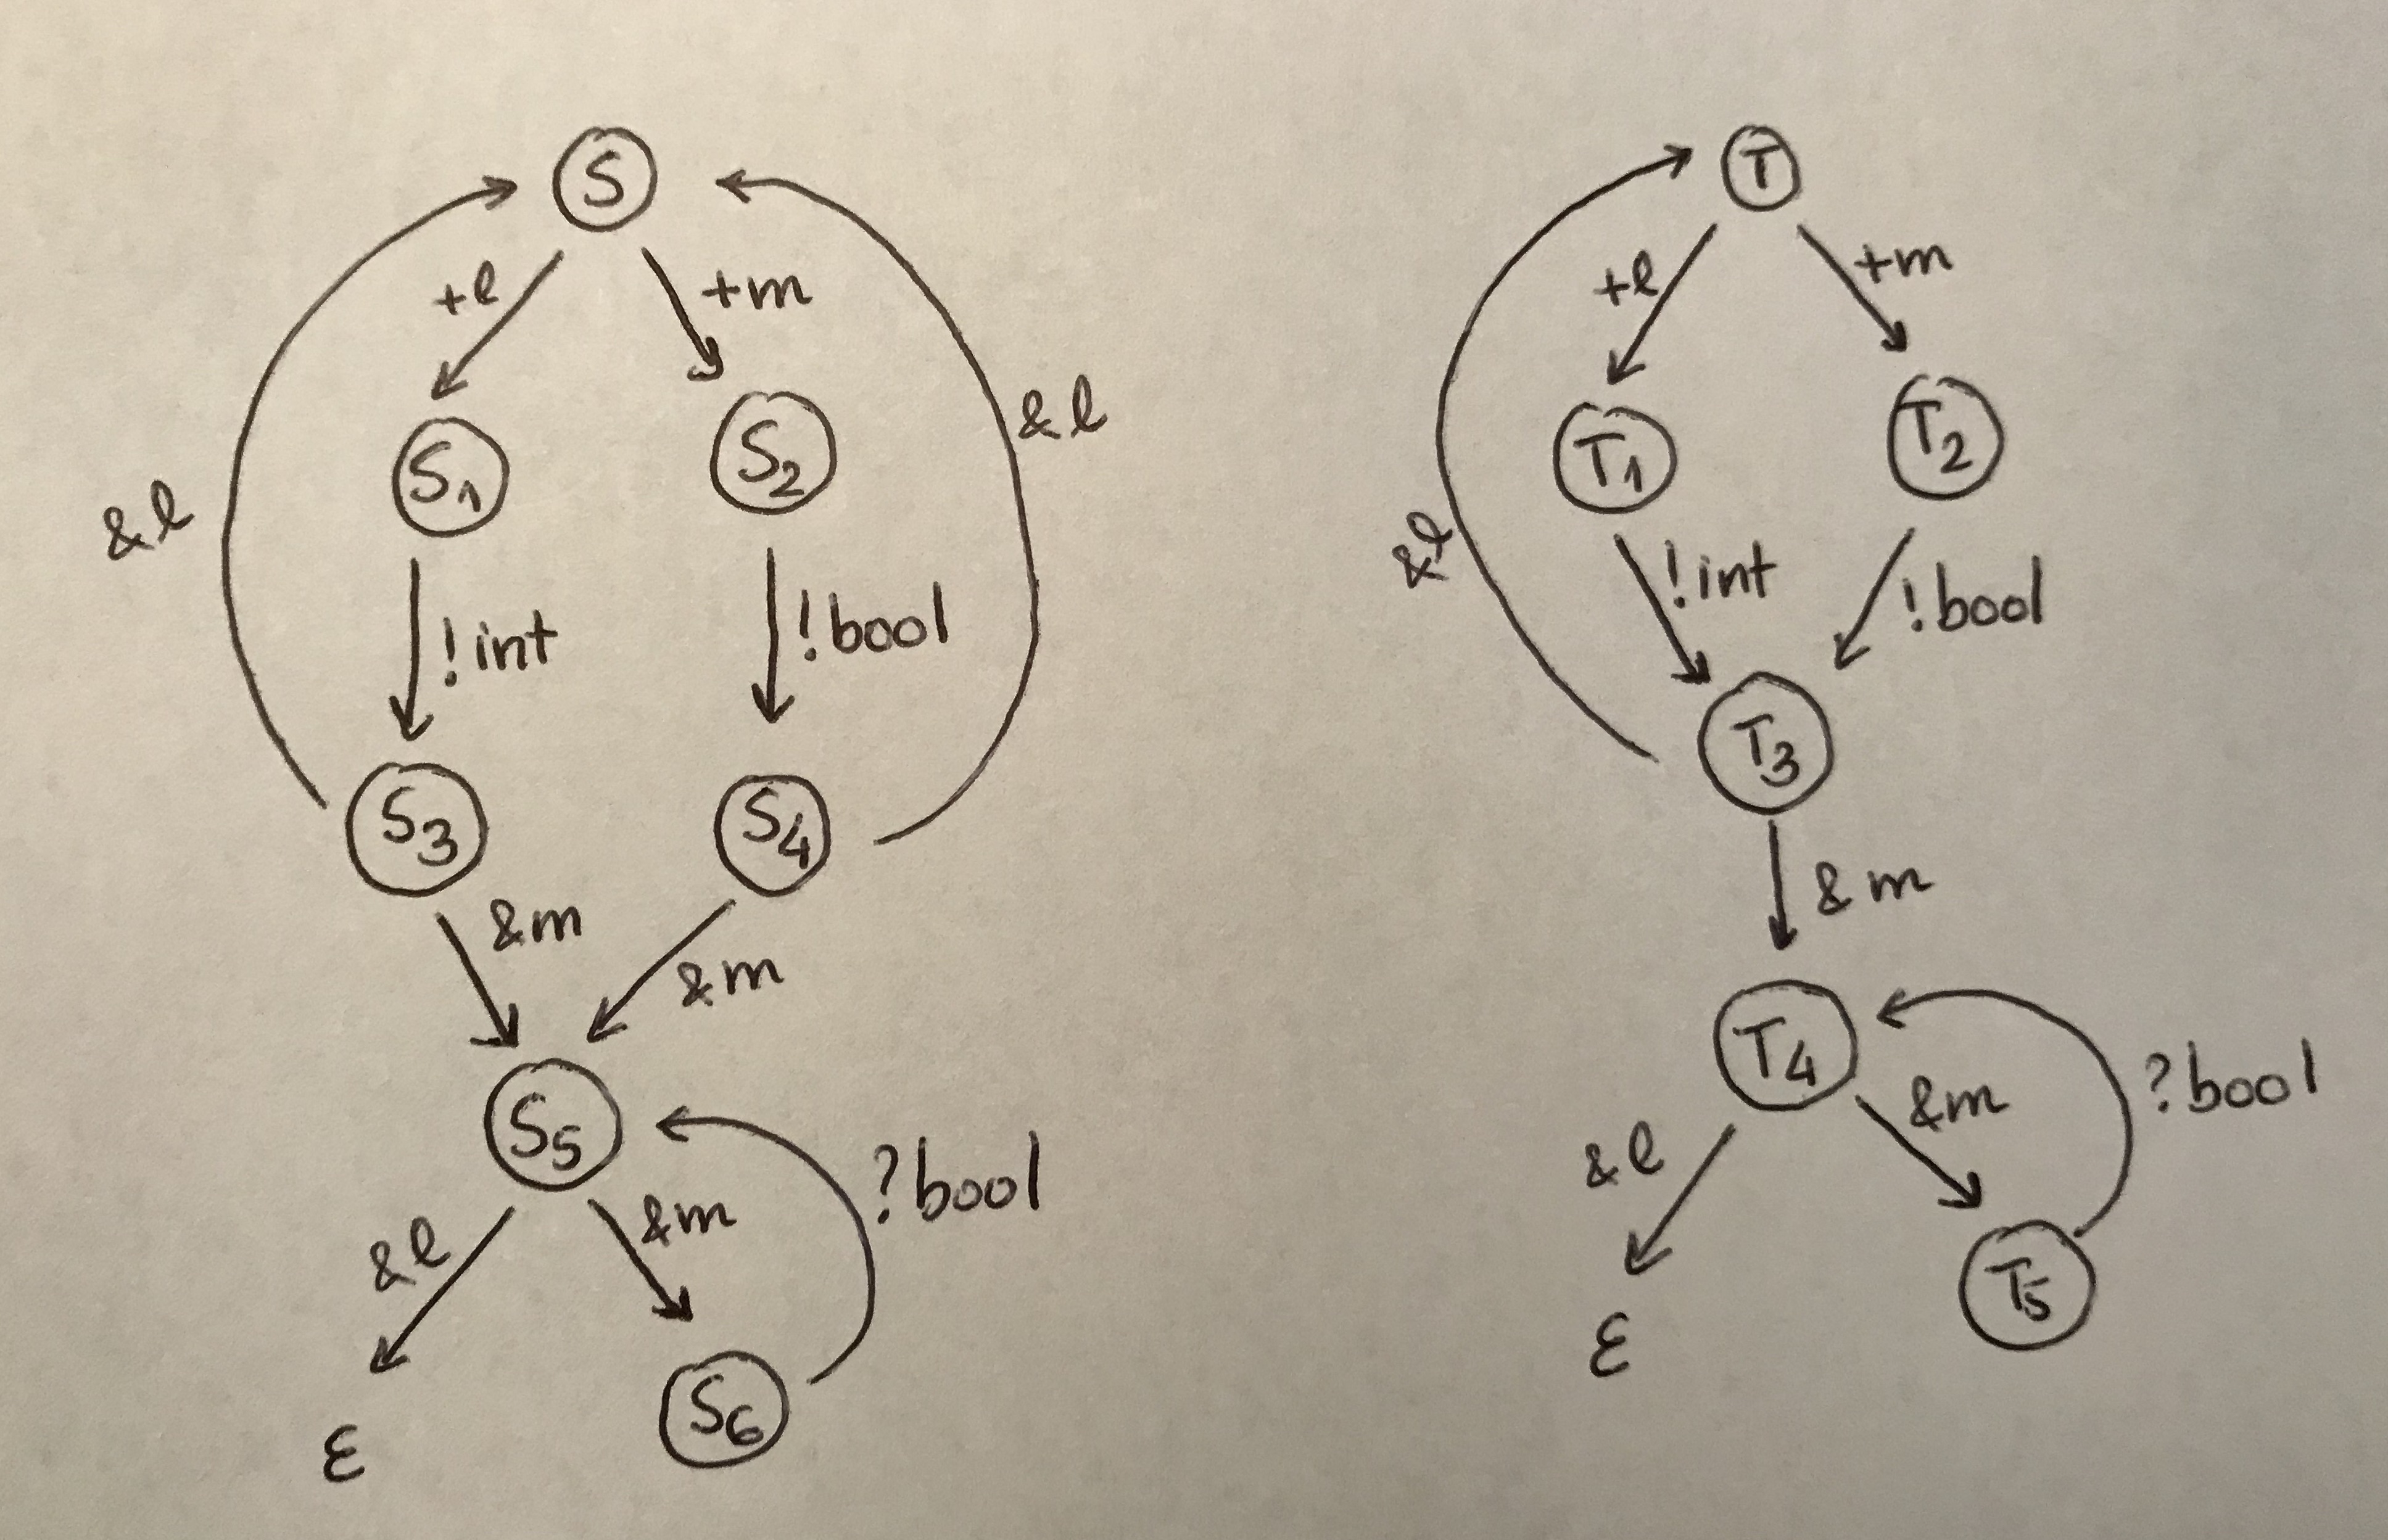
\includegraphics[width=\columnwidth]{PAgraphsST.jpg}
% 		\caption{Process algebra graphs for $S$ and $T$.}
% 			\label{fig:PAgraphsST}
% 	\end{figure}
% 	The algorithm we propose in this work derives the expansion tree for $S\sim T$ as a sequence of nodes. The nodes in this expansion tree can be labeled with a trace of the nodes that lie ahead, based on the syntactical structure of $S$ and $T$. We get the following sequence of labeled nodes in the expansion tree for $S\sim T$:\\\\
% \begin{tikzcd}[cells={nodes={draw=black}}, column sep=large]
%   \enspace (S,T) \enspace \ar[r,"expand"]
% & \enspace  (S_1S_3S_5,T_1T_3), (S_2S_4S_5, T_2T_3) \enspace \ar[r,"expand"]
% & \enspace  (S_3S_5,T_3), (S_4S_5, T_3) \enspace  
% \end{tikzcd} 
% $\xrightarrow{\text{expand}}$\\\\
% \begin{tikzcd}[cells={nodes={draw=black}}, column sep=large]
% & \enspace(SS_5,T),(SS_5,T),(S_5,T_4),(S_5,T_4)  \enspace\ar[r,dashed,"bpa1"]
% &\enspace (S_5,\varepsilon),(S_5,T_4) \enspace 
% \end{tikzcd} 
% $\xrightarrow{\text{expand}}$ \\\\
% \begin{tikzcd}[cells={nodes={draw=black}}, column sep=large]
% &\enspace (S_6S_5,T_5T_4), (\varepsilon,\varepsilon) \enspace \ar[r,dashed,"reflex"] 
% &\enspace (S_6S_5,T_5T_4)\enspace \ar[r,"expand"]
% & \enspace(S_5,T_4)\enspace \ar[r,dashed,"bpa1"]
% &\emptyset\\
% \end{tikzcd}

% 	The process alternates between simplification and expansion operations, denoted by dashed and solid arrows, respectively. Having reached an empty node, we conclude that $S\sim T$.\\\smallskip
	
% 	Now consider the types:
% 	\[ R \triangleq \mu x.\&\{\ell\colon ?\,\boolk;x, m\colon ?\,\intk;x;x \} \text{ and }  U \triangleq \mu x.\&\{\ell\colon ?\,\boolk, m\colon ?\,\intk;x;x\} \enspace .\]
	
% 	$R$ and $U$ are represented as PA graphs as shown in Figure~\ref{fig:PAgraphsRU}.
	
% 	\begin{figure}[h!]
% 	\centering
% 		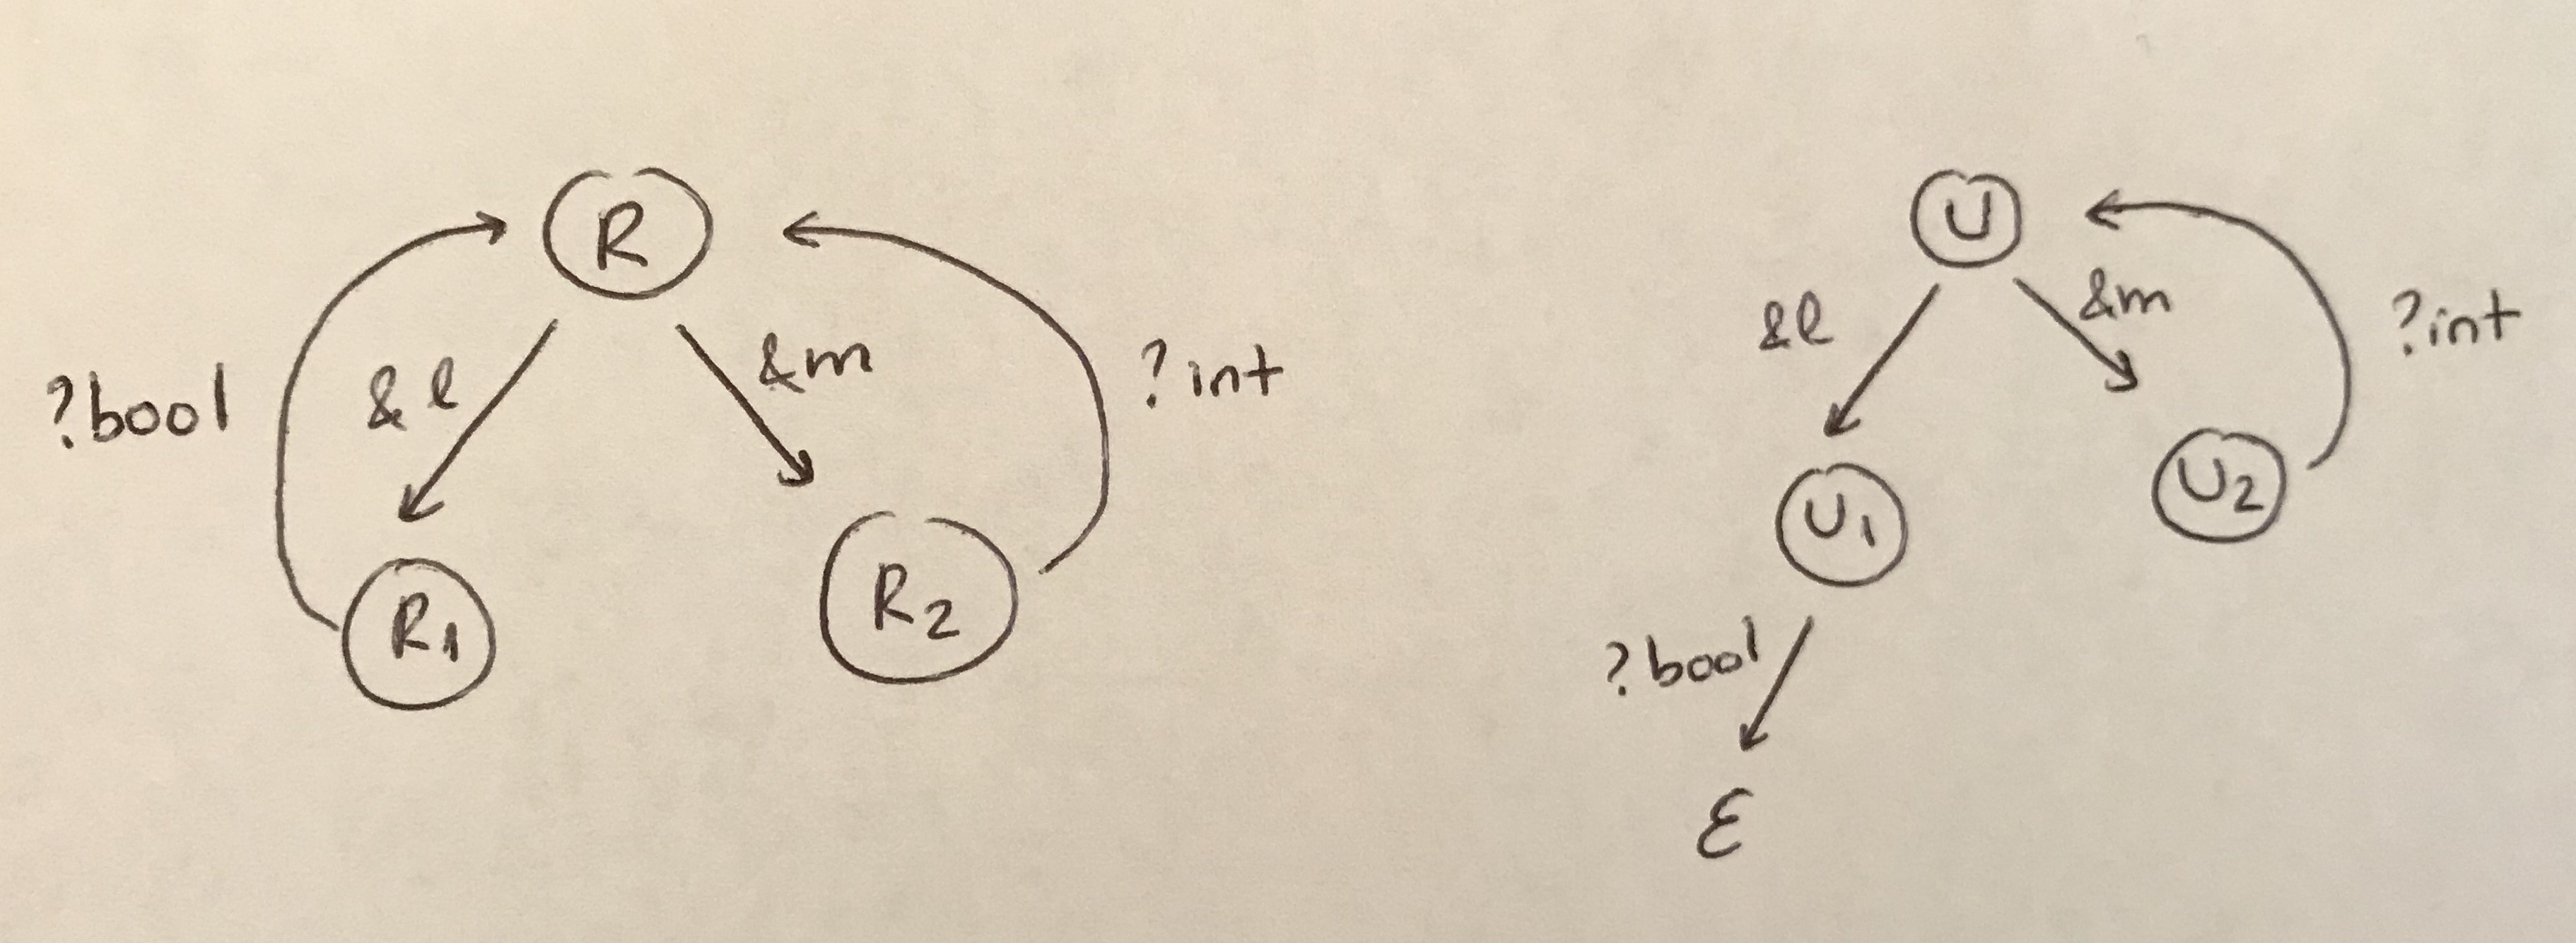
\includegraphics[width=14cm]{PAgraphsRU.jpg}
% 		\caption{Process algebra graphs for $R$ and $U$.}
% 		\label{fig:PAgraphsRU}
% 	\end{figure}
% 	Using the porposed algorithm, we get the following expansion list build upon the syntactical structure of $R$ and $U$ and their representations as PA graphs:\\\\
% \begin{tikzcd}[cells={nodes={draw=black}}, column sep=large]
%   (R,U) \ar[r,"expand"]
% & (R_1 R,U_1), (R_2 R R, U_2 U U) \ar[r,"expand"]
% & (R,\varepsilon), (RR, UU) \ar[r,dashed,"bpa1"] 
% & (R,\varepsilon), (U,\varepsilon) 
% \end{tikzcd} 
% \enspace  $\times$\\\\
% We notice that the last step results from applying BPA1 rule~\cite{janvcar1999techniques} to $(RR,UU)$ knowing that $(R,U)$ is an ancestor node, which leads to the pairs $(R,\varepsilon)$ and $(U,\varepsilon)$. As we then fail to obtain new derived nodes, we decide the type equivalence negatively and conclude that $R\not\sim U$.
% 	\hfill $\triangle$
% \end{example}


%%% Local Variables:
%%% mode: latex
%%% TeX-master: "main"
%%% End:


\end{document}


%%% Local Variables:
%%% mode: latex
%%% TeX-master: t
%%% End:
